\chapter{Experimental Results}
\label{experimental}
\thispagestyle{empty}

\begin{quotation}
{\footnotesize
\noindent{\emph{``Rick: Come on, flip the pickle, Morty. You're not gonna regret it. The payoff is huge.
(Morty hesitantly picks up the screwdriver and turns the pickle over. The pickle has Rick's face on it) I turned myself into a pickle, Morty! Boom! Big reveal: I'm a pickle. What do you think about that? I turned myself into a pickle! W-what are you just staring at me for, bro. I turned myself into a pickle, Morty! \\
Morty: And? \\
Rick: "And"? What more do you want tacked on to this? I turned myself into a pickle, and 9/11 was an inside job?\\
... \\
Morty: I-I'm just trying to figure out why you would do this. Why anyone would do this. \\
Rick: The reason anyone would do this is, if they could, which they can't, would be because they could, which they can't.''}}
\begin{flushright}
Rick and Morty (Season 3, Episode 3)
\end{flushright}
}
\end{quotation}

 


\section{Ship Steering Domain}
We chose ship steering task~\cite{Anderson:1990:CSC:104204.104226} to test the framework. Ship steering has complex low level dynamics due to its continuous state-action space and it is well suited for designing hierarchies. The task was initially studied as a control theory problem~\cite{shipsteeringACD}. Later, \cite{GhavamzadehHierarchicalPG} introduced the problem to machine learning literature and suggested Hierarchical Policy Gradient Algorithms as a solution. 
Ship steering domain is shown in Figure \ref{fig:shipsteeringdomainbig}.

\begin{figure}[t]
      \centering
      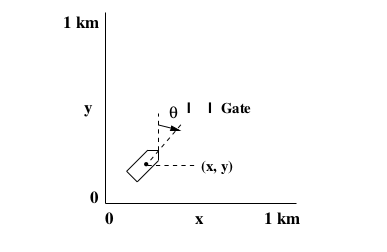
\includegraphics[width = 0.5\textwidth]{./pictures/shipbigenv.png}
      \caption{Ship steering domain}
      \label{fig:shipsteeringdomainbig}
\end{figure}
    
A ship starts at a randomly chosen position, orientation and turning rate and has to be maneuvered at a constant speed through a gate placed at a fixed position in minimum time. Since the ship speed is constant, minimum-time policy is equivalent to shortest-path policy. We consider the ship model given by a set of nonlinear difference equations~\ref{eqn:shipsteeringequation}.

\begin{equation}
\label{eqn:shipsteeringequation}
\begin{split}
     &x\left[t+1 \right] = x[t] + \Delta V \sin \theta \left[t\right]\\
     &y\left[t+1 \right] = y[t] + \Delta V \cos \theta \left[t\right]\\
     &\theta\left[t+1 \right] = \theta[t] + \Delta \dot{\theta} \left[t\right]\\
     &\dot{\theta} \left[t+1\right] =  \dot{\theta} \left[t\right] +\Delta (r\left[t\right] - \dot{\theta}\left[t\right])/T
\end{split}
\end{equation}
where $T = 5$ is the constant time needed to converge to the desired turning rate, $V = 3\frac{m}{s}$ is the constant speed of the ship, and $\Delta = 0.2 s$ is the sampling interval. The control interval is $0.6 s$ (three times the sampling interval).
There is a time lag between changes in the desired turning rate and the actual action, modeling the effects of a real ship’s inertia and the resistance of the water. The state variables are the coordinates ($x$, $y$), the orientation ($\theta$) and the actual turning rate of the ship ($\dot{\theta}$). The control signal is the desired turning rate of the ship ($r$). The state variables and the control signal are continuous within their range given in the table \ref{table:ranges}.

\begin{table}[t]
  \centering
  \begin{tabular}{c r r}
     \toprule
     Variable & Min & Max \\
     \midrule
     $x$ & 0 & 1000 \\ 
     $y$ & 0 & 1000 \\
     $\theta$ & $-\pi$ & $\pi$ \\
     $\dot{\theta}$ & $-\frac{\pi}{12}$ & $\frac{\pi}{12}$ \\
     $r$ & $-\frac{\pi}{12}$ & $\frac{\pi}{12}$ \\
     \bottomrule
  \end{tabular}
  \caption{State and action variable ranges}
  \label{table:ranges}
\end{table}

The ship steering problem is episodic. In each episode, the goal is to learn the sequence of control actions that steer the center of the ship through the gate in the minimum amount of time. To make sure the optimal policy is to find the shortest path, every step of an episode has a reward of -1. If the ship moves out of bound, the episode terminates and is considered as a failure. In this case, environment returns -100 as a reward. The sides of the gate are placed at coordinates (350,400) and (450,400). If the center of the ship passes through the gate, episode ends with a success and a reward 0 is received. 

The task is not simple for classical RL algorithms for several reasons~\cite{GhavamzadehHierarchicalPG}. First, since the ship cannot turn faster than $\frac{\pi}{12} \frac{rad}{s}$, all state variables change only by a small amount at each control interval. Thus, we need a high resolution discretization of the state space in order to accurately model state transitions, which requires a large number of parameters for the function approximator and makes the problem intractable. Second, there is a time lag between changes in the desired turning rate $r$ and the actual turning rate, ship’s position $x$, $y$ and orientation $\theta$, which requires the controller to deal with long delays. In addition, the reward is not much informative. 

Thus, we used a simplified version of the problem for the early experiments. The simplified ship steering domain is given in Figure~\ref{fig:shipsteeringdomain}. The domain boundaries are smaller, to shrink the state space. Ranges of the state and action variables are given in Table~\ref{table:rangessmall}. In this case, the gate is positioned in the upper right corner of the map at the coordinates (100,120) and (120,100). The ship starts at the origin of the state space, i.e., fixed at position (0, 0) with orientation 0 and no angular velocity.   
\begin{figure}[t]
      \centering
      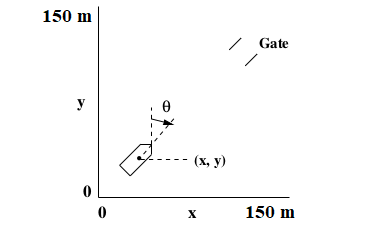
\includegraphics[width = 0.45\textwidth]{./pictures/shipsteeringdomain.png}
      \caption{Ship steering small domain}
      \label{fig:shipsteeringdomain}
\end{figure}

\begin{table}[t]
  \centering
  \begin{tabular}{c r r}
     \toprule
     Variable & Min & Max \\
     \midrule
     $x$ & 0 & 150 \\ 
     $y$ & 0 & 150 \\
     $\theta$ & $-\pi$ & $\pi$ \\
     $\dot{\theta}$ & $-\frac{\pi}{12}$ & $\frac{\pi}{12}$ \\
     $r$ & $-\frac{\pi}{12}$ & $\frac{\pi}{12}$ \\
     \bottomrule
  \end{tabular}
  \caption{State and action variable ranges for small environment}
  \label{table:rangessmall}
\end{table}

\section{Flat Policy Search Algorithms}
Experiments with flat PS algorithms are implemented for the small domain using \texttt{mushroom} library. The flat algorithms use a tiling with three dimensions to divide the state space $5 \times 5 \times 6$ tiles each. 100 experiments have been carried out for each flat algorithm. Every experiment lasted 25 epochs. In every epoch, the learning algorithm runs for 200 episodes. Then the evaluation run is carried out. The resulting dataset of the evaluation run is used to compute cumulative discounted rewards ($\mathcal{J}$) for each episode in the evaluation dataset and averaged for each epoch. With the same method, also the mean length of the episodes for each epoch is computed. These data are averaged for 100 experiments.

For the major part of the experiments, PG algorithms are implemented with an adaptive learning rate. Adaptive learning rate constrains the step of the learning algorithm with a given metric, instead of moving of a step proportional to the gradient. The step rule is given in Equation~\ref{eqn:adaptivelr}. Adaptive learning rate can be used to prevent jumps when the gradient magnitude is big. 

\begin{equation}
\label{eqn:adaptivelr}
    \begin{aligned}
    \Delta\theta=\argmax_{\Delta\vartheta}\Delta\vartheta^{t}\nabla_{\theta}J
    \\
    s.t.:\Delta\vartheta^{T}M\Delta\vartheta\leq\varepsilon
    \end{aligned}
\end{equation} 


GPOMDP, a step-based PG algorithm, has been implemented to learn the parameters of a multivariate Gaussian policy with diagonal standard deviation. The initial standard deviation ($\sigma)$ is set to $3\times10^{-2}$. The mean of the Gaussian is formulated with a linear function approximator with tiles. Learning parameter is adaptive with a value of $10^{-5}$. Policy is fit every 40 episodes during the learning run. Number of episodes of an evaluation run is also 40. 

RWR, REPS and PGPE algorithms work on a distribution of policy parameters and they can be used with deterministic policies. They have been implemented to learn the distribution of the mean $\mu$ of a deterministic policy. Mean is linearly parameterized with the tiles. The distribution is a Gaussian distribution with diagonal standard deviation. The initial mean $\mu$ is the null vector, and $4\times10^{-1}$ variance $\sigma^2$ for every dimension. All three algorithms are run for 200 episodes to learn at each epoch. Every 20 episodes, the distribution parameters are updated. The evaluation run lasts 20 episodes. The learning rate of PGPE is adaptive and the value is initially set to $1.5$. REPS and RWR do not require the learning rate to be specified as explained in Chapter~\ref{stateoftheart}. REPS is used with a max KL step $\epsilon = 1$, and RWR with a constant $\beta = 0.7$ for the exponential transformation. 

\section{Hierarchical Block Diagram Approach}

The ship steering control system consists fundamentally of two parts~\cite{shipsteeringACD}:
 
\begin{itemize}
   \item a ship autopilot which automatically manipulates the rudder to decrease the error between the reference heading angle and the actual heading angle, and
   \item an operator, either human or a machine, that closes up the control loop given the reference angles to follow a desired trajectory on the ocean.
\end{itemize}

The control theory approach to ship steering problem is preserved for the subtask definitions with our framework. The corresponding block diagram is given in Figure~\ref{fig:blockdiagramship}. 

\begin{figure}[t] 
      \centering
      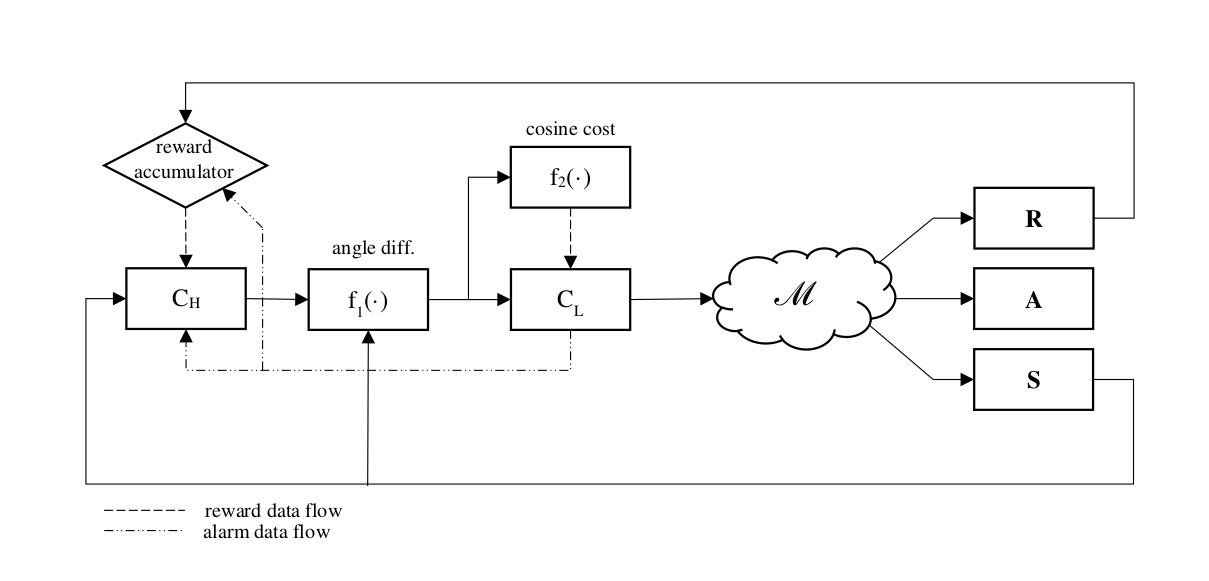
\includegraphics[width = \textwidth]{./pictures/blockdiagramshipsteering.png}
      \caption{HRL block diagram for ship steering task}
      \label{fig:blockdiagramship}
\end{figure} 

Low level controller learns to approximate the optimal policy to decrease the error between the reference angle and the actual angle.  High level controller learns to drive the low level by producing reference positions in the map that approximate the shortest paths to the gate. A function block in between the control blocks ($f_1( \cdot )$) computes the reference angle for the low level, given the reference position and the states. The performance metric of the high level control is the extrinsic reward, whereas the one of the low level is computed by another function block, $f_2( \cdot )$. $f_2( \cdot )$ returns the cosine of the angle difference computed by $f_1( \cdot )$. As the difference of the reference angle and the actual angle gets close to 0, the reward advances to 1 and as it grows, the reward decreases to -1. 

When the low level controller finishes its episode, it raises an alarm for the high level. In the following cycle, a new reference point is estimated for the level. The same alarm signal is passed to the reward accumulator of the high level controller with the motivations described in Chapter~\ref{proposed}. 

The high level controller uses the GPOMDP algorithm to learn a multivariate Gaussian policy with diagonal standard deviation. Its mean is initialized in the middle of the map, that is $(75, 75)$, for the small domain. The variance of both dimensions is $40$. The algorithm fits every 20 episodes with an adaptive learning rate of 10. Horizon is 100 steps for both controllers.

Low level control policy should steer the ship in the direction of the angle error. That is, if the reference angle is larger than the current angle, angular velocity output of the low level control should be positive and vice versa. Low level controller is first tested with a GPOMDP algorithm with a differentiable parameterized policy such as a linear one given as $\pi(x) = \omega x$, where $x$ is the error $\Delta\theta$ over the angle. In this scheme, the parameters of the low level policy are expected to be positive to make sure that the input error and the output angular velocity have the same sign. However, when the high level policy is not reliable, low level policy may choose to go outside of the map to finish the episode quickly. In addition, when the optimal parameter is lower than the current one, a big gradient step may cause trespassing the 0 limit, which results in instability. 
To ensure stability, the parameter of the policy needs to be forced to have a positive value. This can be achieved with a deterministic policy by using the absolute values of  weights, that is,  $\pi(x) = \left|\omega\right|x$. However, this policy is not differentiable. Therefore, classical PG algorithms cannot be exploited. Thus, the low level controller uses a black box optimization method. PGPE algorithm learns the distribution of the weights of a non-differentiable deterministic policy. The distribution over the weights has zero mean and $10^{-3}$ as variance initially. The algorithm fits at every 10 episode of the low level controller. The action taken by the low level is indeed a proportional control action. The error signal is multiplied by a constant, $K_P$. The distribution over $K_P$ is learned by the PGPE algorithm. An adaptive learning rate is used with a value $5\times10{-4}$.

Another experimental setup is constructed in which the low level control applies also the integral action. To achieve this, an error accumulator block is added between $f_1( \cdot )$ and the low level controller as shown in Figure~\ref{fig:shipsteeringpi}.

\begin{figure}[t]
      \centering
      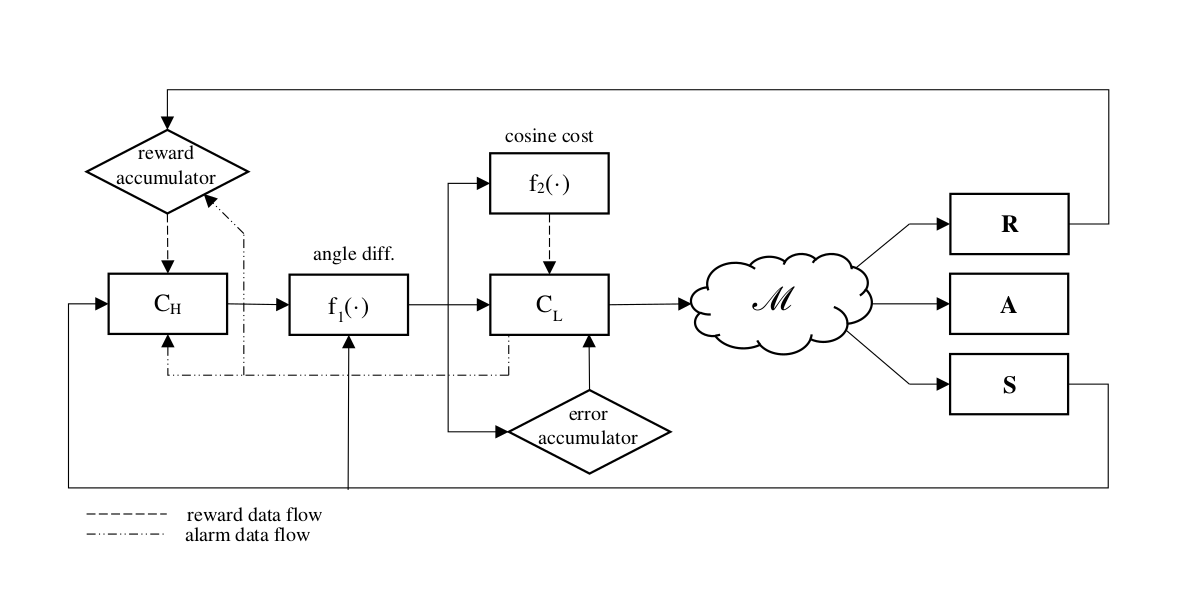
\includegraphics[width = \textwidth]{./pictures/pishipsteering.png}
      \caption{HRL block diagram for ship steering task, PI control action}
      \label{fig:shipsteeringpi}
\end{figure}

 In this case, the state of the low level control is two dimensional. The adopted deterministic policy is $\pi(x) = \left|\boldsymbol{\omega}^T\right|x$. The state vector is $x=\left[\Delta\theta, \int\Delta\theta dt\right]$. The parameter vector is $\boldsymbol{\omega}=\left[K_P, K_I\right]$, where the $K_P$ parameter corresponds to the proportional gain, and the $K_I$ parameter is the integral gain, as they multiply the error and the integral of the error respectively.


\section{Results in Small Domain}

Results of the flat algorithms and of the hierarchical schemes designed with the block diagram approach are compared. 

Figure~\ref{fig:art_J} shows the mean of the objective function for every epoch, averaged for 100 experiments for each algorithm. It shows that flat PG algorithms, i.e., PGPE and GPOMDP, converge much more slowly than the other ones. This is due to the fact that for these algorithms learning rate should be defined. If the learning rate is low, the convergence is slow and if it is too high, learning may be unstable. 

\begin{figure}[t!]
	\centering
    \vspace{-1.0 cm}
    \setlength\figureheight{5.5cm}  
	\setlength\figurewidth{.9\textwidth}
	% This file was created by matplotlib2tikz v0.6.16.
\begin{tikzpicture}

\definecolor{color0}{rgb}{0,0.75,0.75}
\definecolor{color1}{rgb}{0.75,0,0.75}

\begin{axis}[
xlabel={epoch},
ylabel={J},
xmin=-1.25, xmax=26.25,
ymin=-102.045722411051, ymax=-57.2134804981018,
width=\figurewidth,
height=\figureheight,
tick align=outside,
tick pos=left,
x grid style={white!69.01960784313725!black},
y grid style={white!69.01960784313725!black},
legend cell align={left},
legend entries={{H-PGPE},{REPS},{RWR},{PGPE},{GPOMDP}},
legend style={at={(0.97,0.03)}, anchor=south east, draw=white!80.0!black}
]
\addlegendimage{no markers, blue}
\addlegendimage{no markers, red}
\addlegendimage{no markers, green!50.0!black}
\addlegendimage{no markers, color0}
\addlegendimage{no markers, color1}
\path [draw=blue, semithick] (axis cs:0,-100)
--(axis cs:0,-100);

\path [draw=blue, semithick] (axis cs:1,-93.8844031073029)
--(axis cs:1,-95.009392845152);

\path [draw=blue, semithick] (axis cs:2,-92.988679778882)
--(axis cs:2,-94.455724491924);

\path [draw=blue, semithick] (axis cs:3,-89.4770390462373)
--(axis cs:3,-91.5626994845177);

\path [draw=blue, semithick] (axis cs:4,-83.5113933816678)
--(axis cs:4,-86.4362909181087);

\path [draw=blue, semithick] (axis cs:5,-77.4891101370856)
--(axis cs:5,-80.8815692290756);

\path [draw=blue, semithick] (axis cs:6,-71.3979405955427)
--(axis cs:6,-74.5860307612094);

\path [draw=blue, semithick] (axis cs:7,-66.9352745847397)
--(axis cs:7,-70.3229400593475);

\path [draw=blue, semithick] (axis cs:8,-64.5097641964084)
--(axis cs:8,-67.1651054669046);

\path [draw=blue, semithick] (axis cs:9,-62.7616953407986)
--(axis cs:9,-65.3071722033568);

\path [draw=blue, semithick] (axis cs:10,-60.8098074053026)
--(axis cs:10,-62.6421477011409);

\path [draw=blue, semithick] (axis cs:11,-60.9643522984729)
--(axis cs:11,-62.8315185481412);

\path [draw=blue, semithick] (axis cs:12,-60.7362863275358)
--(axis cs:12,-62.430110564971);

\path [draw=blue, semithick] (axis cs:13,-60.3316662413563)
--(axis cs:13,-62.0075482576081);

\path [draw=blue, semithick] (axis cs:14,-59.8101477589761)
--(axis cs:14,-61.2360357577435);

\path [draw=blue, semithick] (axis cs:15,-59.3545994981829)
--(axis cs:15,-60.5245326920989);

\path [draw=blue, semithick] (axis cs:16,-59.9492448417058)
--(axis cs:16,-61.7625818956256);

\path [draw=blue, semithick] (axis cs:17,-59.8445548849395)
--(axis cs:17,-61.1828533442119);

\path [draw=blue, semithick] (axis cs:18,-59.6474778394595)
--(axis cs:18,-61.1941864966046);

\path [draw=blue, semithick] (axis cs:19,-59.6472124838335)
--(axis cs:19,-61.0492925768536);

\path [draw=blue, semithick] (axis cs:20,-59.2523141432313)
--(axis cs:20,-60.1308671855049);

\path [draw=blue, semithick] (axis cs:21,-59.6150564558487)
--(axis cs:21,-60.7430263266553);

\path [draw=blue, semithick] (axis cs:22,-59.479005102806)
--(axis cs:22,-60.8607910312466);

\path [draw=blue, semithick] (axis cs:23,-59.496371057599)
--(axis cs:23,-60.6035422311425);

\path [draw=blue, semithick] (axis cs:24,-59.2513096759631)
--(axis cs:24,-59.8708681188255);

\path [draw=blue, semithick] (axis cs:25,-59.576033041729)
--(axis cs:25,-60.7148514397126);

\path [draw=red, semithick] (axis cs:0,-99.340938091202)
--(axis cs:0,-99.6765177904523);

\path [draw=red, semithick] (axis cs:1,-86.9696915058598)
--(axis cs:1,-91.2842458346257);

\path [draw=red, semithick] (axis cs:2,-70.5203134016048)
--(axis cs:2,-75.3827222086141);

\path [draw=red, semithick] (axis cs:3,-64.609782600434)
--(axis cs:3,-69.0890476554475);

\path [draw=red, semithick] (axis cs:4,-62.7412132718815)
--(axis cs:4,-66.8617231101294);

\path [draw=red, semithick] (axis cs:5,-61.493938772641)
--(axis cs:5,-65.266381187646);

\path [draw=red, semithick] (axis cs:6,-60.9080955761437)
--(axis cs:6,-64.2382385271308);

\path [draw=red, semithick] (axis cs:7,-60.7036473598561)
--(axis cs:7,-63.8902712352318);

\path [draw=red, semithick] (axis cs:8,-60.5440366495401)
--(axis cs:8,-63.7042865629365);

\path [draw=red, semithick] (axis cs:9,-60.5540153114945)
--(axis cs:9,-63.7368389825067);

\path [draw=red, semithick] (axis cs:10,-60.4617134875305)
--(axis cs:10,-63.61971422531);

\path [draw=red, semithick] (axis cs:11,-60.4391637879797)
--(axis cs:11,-63.5985499551863);

\path [draw=red, semithick] (axis cs:12,-60.4784505290768)
--(axis cs:12,-63.638308638653);

\path [draw=red, semithick] (axis cs:13,-60.4382160833601)
--(axis cs:13,-63.597604703527);

\path [draw=red, semithick] (axis cs:14,-60.437790368404)
--(axis cs:14,-63.5972250018576);

\path [draw=red, semithick] (axis cs:15,-60.4381349246686)
--(axis cs:15,-63.5976015659084);

\path [draw=red, semithick] (axis cs:16,-60.437575365644)
--(axis cs:16,-63.5970352726449);

\path [draw=red, semithick] (axis cs:17,-60.4558709663328)
--(axis cs:17,-63.6164633366484);

\path [draw=red, semithick] (axis cs:18,-60.4589820572708)
--(axis cs:18,-63.6168911671207);

\path [draw=red, semithick] (axis cs:19,-60.4381931180551)
--(axis cs:19,-63.597603586875);

\path [draw=red, semithick] (axis cs:20,-60.437575365644)
--(axis cs:20,-63.5970352726449);

\path [draw=red, semithick] (axis cs:21,-60.4585706043821)
--(axis cs:21,-63.6165132311746);

\path [draw=red, semithick] (axis cs:22,-60.437790368404)
--(axis cs:22,-63.5972250018576);

\path [draw=red, semithick] (axis cs:23,-60.45859160974)
--(axis cs:23,-63.6168969577894);

\path [draw=red, semithick] (axis cs:24,-60.4781612401401)
--(axis cs:24,-63.6373798446298);

\path [draw=red, semithick] (axis cs:25,-60.437575365644)
--(axis cs:25,-63.5970352726449);

\path [draw=green!50.0!black, semithick] (axis cs:0,-99.1581387340433)
--(axis cs:0,-99.5481090039911);

\path [draw=green!50.0!black, semithick] (axis cs:1,-80.026635650284)
--(axis cs:1,-85.727121653856);

\path [draw=green!50.0!black, semithick] (axis cs:2,-68.9581863025615)
--(axis cs:2,-73.7213317906966);

\path [draw=green!50.0!black, semithick] (axis cs:3,-65.6956570461768)
--(axis cs:3,-69.9017474993277);

\path [draw=green!50.0!black, semithick] (axis cs:4,-64.1527761758554)
--(axis cs:4,-68.0739174150851);

\path [draw=green!50.0!black, semithick] (axis cs:5,-63.9124984991473)
--(axis cs:5,-67.7846857212685);

\path [draw=green!50.0!black, semithick] (axis cs:6,-63.6743095240205)
--(axis cs:6,-67.5856396425221);

\path [draw=green!50.0!black, semithick] (axis cs:7,-63.2868403376964)
--(axis cs:7,-67.167590915216);

\path [draw=green!50.0!black, semithick] (axis cs:8,-63.3108371629945)
--(axis cs:8,-67.1899199040878);

\path [draw=green!50.0!black, semithick] (axis cs:9,-63.0436749190446)
--(axis cs:9,-66.8795370874546);

\path [draw=green!50.0!black, semithick] (axis cs:10,-62.940045094149)
--(axis cs:10,-66.7690052137587);

\path [draw=green!50.0!black, semithick] (axis cs:11,-62.9508682431492)
--(axis cs:11,-66.7927823215623);

\path [draw=green!50.0!black, semithick] (axis cs:12,-62.9149898808233)
--(axis cs:12,-66.7479361202862);

\path [draw=green!50.0!black, semithick] (axis cs:13,-62.8972913868626)
--(axis cs:13,-66.7356527821435);

\path [draw=green!50.0!black, semithick] (axis cs:14,-62.8596476680646)
--(axis cs:14,-66.7061153537228);

\path [draw=green!50.0!black, semithick] (axis cs:15,-62.8150857558692)
--(axis cs:15,-66.6647303665289);

\path [draw=green!50.0!black, semithick] (axis cs:16,-62.8001270486436)
--(axis cs:16,-66.6445437146755);

\path [draw=green!50.0!black, semithick] (axis cs:17,-62.7960659371176)
--(axis cs:17,-66.6409986224146);

\path [draw=green!50.0!black, semithick] (axis cs:18,-62.7944993351245)
--(axis cs:18,-66.6398571879558);

\path [draw=green!50.0!black, semithick] (axis cs:19,-62.8040224822818)
--(axis cs:19,-66.6541258617261);

\path [draw=green!50.0!black, semithick] (axis cs:20,-62.7917446454782)
--(axis cs:20,-66.6373856247019);

\path [draw=green!50.0!black, semithick] (axis cs:21,-62.7914966359793)
--(axis cs:21,-66.6371982247025);

\path [draw=green!50.0!black, semithick] (axis cs:22,-62.7901516933118)
--(axis cs:22,-66.6357265126988);

\path [draw=green!50.0!black, semithick] (axis cs:23,-62.7901628954246)
--(axis cs:23,-66.6356428053543);

\path [draw=green!50.0!black, semithick] (axis cs:24,-62.7872626927784)
--(axis cs:24,-66.6329665347076);

\path [draw=green!50.0!black, semithick] (axis cs:25,-62.788210241327)
--(axis cs:25,-66.6339829243369);

\path [draw=color0, semithick] (axis cs:0,-99.0619646721375)
--(axis cs:0,-99.4831354500871);

\path [draw=color0, semithick] (axis cs:1,-98.3106370090467)
--(axis cs:1,-98.9810074991301);

\path [draw=color0, semithick] (axis cs:2,-97.3460617668763)
--(axis cs:2,-98.2888480707866);

\path [draw=color0, semithick] (axis cs:3,-97.4688706837659)
--(axis cs:3,-98.3938385676808);

\path [draw=color0, semithick] (axis cs:4,-96.8657939469452)
--(axis cs:4,-97.8956649883799);

\path [draw=color0, semithick] (axis cs:5,-95.8152813951146)
--(axis cs:5,-97.2212870397311);

\path [draw=color0, semithick] (axis cs:6,-93.9069801391457)
--(axis cs:6,-96.2531543992857);

\path [draw=color0, semithick] (axis cs:7,-92.0622529701026)
--(axis cs:7,-94.9835503652816);

\path [draw=color0, semithick] (axis cs:8,-90.2299421160219)
--(axis cs:8,-93.3782156372657);

\path [draw=color0, semithick] (axis cs:9,-87.4518528563457)
--(axis cs:9,-91.439121205612);

\path [draw=color0, semithick] (axis cs:10,-85.5990407286016)
--(axis cs:10,-89.7802831095007);

\path [draw=color0, semithick] (axis cs:11,-82.9871730359104)
--(axis cs:11,-87.3122043760532);

\path [draw=color0, semithick] (axis cs:12,-80.1602801674897)
--(axis cs:12,-85.0907541405663);

\path [draw=color0, semithick] (axis cs:13,-77.6687532958262)
--(axis cs:13,-82.7730378844951);

\path [draw=color0, semithick] (axis cs:14,-77.3360414376375)
--(axis cs:14,-82.374570928434);

\path [draw=color0, semithick] (axis cs:15,-76.1292874116903)
--(axis cs:15,-81.092685861246);

\path [draw=color0, semithick] (axis cs:16,-73.3554848940945)
--(axis cs:16,-78.2353976662902);

\path [draw=color0, semithick] (axis cs:17,-71.6159770142584)
--(axis cs:17,-76.2407043928117);

\path [draw=color0, semithick] (axis cs:18,-70.7060994018115)
--(axis cs:18,-75.1672745242444);

\path [draw=color0, semithick] (axis cs:19,-68.4123756884912)
--(axis cs:19,-72.6687922085187);

\path [draw=color0, semithick] (axis cs:20,-69.0173877575832)
--(axis cs:20,-73.2744772073133);

\path [draw=color0, semithick] (axis cs:21,-67.9647516378067)
--(axis cs:21,-72.0866857228954);

\path [draw=color0, semithick] (axis cs:22,-67.8362160703379)
--(axis cs:22,-71.8738590635436);

\path [draw=color0, semithick] (axis cs:23,-66.8820099408885)
--(axis cs:23,-70.8623854022783);

\path [draw=color0, semithick] (axis cs:24,-66.9736563310659)
--(axis cs:24,-70.947381494199);

\path [draw=color0, semithick] (axis cs:25,-66.0805566543473)
--(axis cs:25,-69.7427805434904);

\path [draw=color1, semithick] (axis cs:0,-100)
--(axis cs:0,-100);

\path [draw=color1, semithick] (axis cs:1,-100)
--(axis cs:1,-100);

\path [draw=color1, semithick] (axis cs:2,-100)
--(axis cs:2,-100);

\path [draw=color1, semithick] (axis cs:3,-99.952238643842)
--(axis cs:3,-100.007893233189);

\path [draw=color1, semithick] (axis cs:4,-99.6687922980591)
--(axis cs:4,-99.8958298484505);

\path [draw=color1, semithick] (axis cs:5,-97.318162989726)
--(axis cs:5,-98.3189864525242);

\path [draw=color1, semithick] (axis cs:6,-88.651116406238)
--(axis cs:6,-90.5252875708918);

\path [draw=color1, semithick] (axis cs:7,-80.1672649149436)
--(axis cs:7,-82.2887325690676);

\path [draw=color1, semithick] (axis cs:8,-75.8331889994754)
--(axis cs:8,-78.1913700213266);

\path [draw=color1, semithick] (axis cs:9,-73.0096915857288)
--(axis cs:9,-75.8144321506643);

\path [draw=color1, semithick] (axis cs:10,-72.2615331925637)
--(axis cs:10,-75.862510531929);

\path [draw=color1, semithick] (axis cs:11,-71.7879776683749)
--(axis cs:11,-76.1357100911378);

\path [draw=color1, semithick] (axis cs:12,-71.6242876833618)
--(axis cs:12,-76.2560728203333);

\path [draw=color1, semithick] (axis cs:13,-71.6977081137204)
--(axis cs:13,-76.6082808676356);

\path [draw=color1, semithick] (axis cs:14,-70.8802098794888)
--(axis cs:14,-76.1488444736344);

\path [draw=color1, semithick] (axis cs:15,-70.6328735103907)
--(axis cs:15,-75.8250122415561);

\path [draw=color1, semithick] (axis cs:16,-69.9444530175129)
--(axis cs:16,-75.2671155368463);

\path [draw=color1, semithick] (axis cs:17,-69.6583132925062)
--(axis cs:17,-75.2366608359157);

\path [draw=color1, semithick] (axis cs:18,-68.7821934875945)
--(axis cs:18,-74.3086194340845);

\path [draw=color1, semithick] (axis cs:19,-69.8921619909389)
--(axis cs:19,-75.6280350506968);

\path [draw=color1, semithick] (axis cs:20,-68.9738249178168)
--(axis cs:20,-74.8222538052091);

\path [draw=color1, semithick] (axis cs:21,-68.8283746083754)
--(axis cs:21,-74.3421208939666);

\path [draw=color1, semithick] (axis cs:22,-68.8095254257202)
--(axis cs:22,-74.5120469067668);

\path [draw=color1, semithick] (axis cs:23,-69.8376351737108)
--(axis cs:23,-75.7269227645284);

\path [draw=color1, semithick] (axis cs:24,-70.7034283224342)
--(axis cs:24,-76.8446793761747);

\path [draw=color1, semithick] (axis cs:25,-70.2978965986904)
--(axis cs:25,-76.4344123547215);

\addplot [semithick, blue, forget plot]
table {%
0 -100
1 -94.4468979762275
2 -93.722202135403
3 -90.5198692653775
4 -84.9738421498883
5 -79.1853396830806
6 -72.9919856783761
7 -68.6291073220436
8 -65.8374348316565
9 -64.0344337720777
10 -61.7259775532218
11 -61.8979354233071
12 -61.5831984462534
13 -61.1696072494822
14 -60.5230917583598
15 -59.9395660951409
16 -60.8559133686657
17 -60.5137041145757
18 -60.420832168032
19 -60.3482525303436
20 -59.6915906643681
21 -60.179041391252
22 -60.1698980670263
23 -60.0499566443707
24 -59.5610888973943
25 -60.1454422407208
};
\addplot [semithick, red, forget plot]
table {%
0 -99.5087279408272
1 -89.1269686702427
2 -72.9515178051095
3 -66.8494151279408
4 -64.8014681910055
5 -63.3801599801435
6 -62.5731670516373
7 -62.296959297544
8 -62.1241616062383
9 -62.1454271470006
10 -62.0407138564202
11 -62.018856871583
12 -62.0583795838649
13 -62.0179103934436
14 -62.0175076851308
15 -62.0178682452885
16 -62.0173053191444
17 -62.0361671514906
18 -62.0379366121957
19 -62.017898352465
20 -62.0173053191444
21 -62.0375419177783
22 -62.0175076851308
23 -62.0377442837647
24 -62.057770542385
25 -62.0173053191444
};
\addplot [semithick, green!50.0!black, forget plot]
table {%
0 -99.3531238690172
1 -82.87687865207
2 -71.339759046629
3 -67.7987022727522
4 -66.1133467954703
5 -65.8485921102079
6 -65.6299745832713
7 -65.2272156264562
8 -65.2503785335412
9 -64.9616060032496
10 -64.8545251539538
11 -64.8718252823557
12 -64.8314630005548
13 -64.816472084503
14 -64.7828815108937
15 -64.739908061199
16 -64.7223353816595
17 -64.7185322797661
18 -64.7171782615401
19 -64.7290741720039
20 -64.7145651350901
21 -64.7143474303409
22 -64.7129391030053
23 -64.7129028503895
24 -64.710114613743
25 -64.7110965828319
};
\addplot [semithick, color0, forget plot]
table {%
0 -99.2725500611123
1 -98.6458222540884
2 -97.8174549188314
3 -97.9313546257234
4 -97.3807294676625
5 -96.5182842174229
6 -95.0800672692157
7 -93.5229016676921
8 -91.8040788766438
9 -89.4454870309788
10 -87.6896619190511
11 -85.1496887059818
12 -82.625517154028
13 -80.2208955901606
14 -79.8553061830358
15 -78.6109866364681
16 -75.7954412801923
17 -73.9283407035351
18 -72.9366869630279
19 -70.5405839485049
20 -71.1459324824483
21 -70.0257186803511
22 -69.8550375669408
23 -68.8721976715834
24 -68.9605189126324
25 -67.9116685989188
};
\addplot [semithick, color1, forget plot]
table {%
0 -100
1 -100
2 -100
3 -99.9800659385157
4 -99.7823110732548
5 -97.8185747211251
6 -89.5882019885649
7 -81.2279987420056
8 -77.012279510401
9 -74.4120618681966
10 -74.0620218622463
11 -73.9618438797563
12 -73.9401802518475
13 -74.152994490678
14 -73.5145271765616
15 -73.2289428759734
16 -72.6057842771796
17 -72.4474870642109
18 -71.5454064608395
19 -72.7600985208178
20 -71.8980393615129
21 -71.585247751171
22 -71.6607861662435
23 -72.7822789691196
24 -73.7740538493045
25 -73.3661544767059
};
\end{axis}

\end{tikzpicture}
    \caption[J comparison, hierarchical vs. flat, small environment]{Comparison of the hierarchical structure w.r.t. flat policy search for small environment. Mean values of objective functions with 95\% confidence intervals are shown}
    \label{fig:art_J}
\end{figure} 

\begin{figure}[t!]
	\centering
	\setlength\figureheight{5.5cm}  
	\setlength\figurewidth{.9\textwidth}
	% This file was created by matplotlib2tikz v0.6.16.
\begin{tikzpicture}

\definecolor{color0}{rgb}{0,0.75,0.75}
\definecolor{color1}{rgb}{0.75,0,0.75}

\begin{axis}[
xlabel={epoch},
ylabel={episode length},
xmin=-1.25, xmax=26.25,
ymin=10.7311004140636, ymax=222.739277592819,
width=\figurewidth,
height=\figureheight,
tick align=outside,
tick pos=left,
x grid style={white!69.01960784313725!black},
y grid style={white!69.01960784313725!black}
]
\path [draw=red, semithick] (axis cs:0,77.6465189830409)
--(axis cs:0,51.6534810169591);

\path [draw=red, semithick] (axis cs:1,132.95882663092)
--(axis cs:1,99.2901733690802);

\path [draw=red, semithick] (axis cs:2,120.533846588516)
--(axis cs:2,95.0331534114837);

\path [draw=red, semithick] (axis cs:3,112.867854818109)
--(axis cs:3,91.2051451818911);

\path [draw=red, semithick] (axis cs:4,94.9615444848637)
--(axis cs:4,86.7604555151364);

\path [draw=red, semithick] (axis cs:5,93.0931087223105)
--(axis cs:5,85.5778912776895);

\path [draw=red, semithick] (axis cs:6,93.0077444511953)
--(axis cs:6,85.3612555488048);

\path [draw=red, semithick] (axis cs:7,92.9470953640859)
--(axis cs:7,85.3619046359141);

\path [draw=red, semithick] (axis cs:8,92.5339966898285)
--(axis cs:8,85.0670033101715);

\path [draw=red, semithick] (axis cs:9,92.4850876831196)
--(axis cs:9,85.0389123168804);

\path [draw=red, semithick] (axis cs:10,92.416308064436)
--(axis cs:10,84.982691935564);

\path [draw=red, semithick] (axis cs:11,92.3791790969445)
--(axis cs:11,84.9488209030555);

\path [draw=red, semithick] (axis cs:12,92.3994425049658)
--(axis cs:12,84.9675574950343);

\path [draw=red, semithick] (axis cs:13,92.3764654773029)
--(axis cs:13,84.9465345226971);

\path [draw=red, semithick] (axis cs:14,92.3754452554255)
--(axis cs:14,84.9455547445745);

\path [draw=red, semithick] (axis cs:15,92.3765778785328)
--(axis cs:15,84.9464221214672);

\path [draw=red, semithick] (axis cs:16,92.3749379505262)
--(axis cs:16,84.9450620494738);

\path [draw=red, semithick] (axis cs:17,92.3842350365168)
--(axis cs:17,84.9527649634832);

\path [draw=red, semithick] (axis cs:18,92.3861705601554)
--(axis cs:18,84.9558294398446);

\path [draw=red, semithick] (axis cs:19,92.3764927750571)
--(axis cs:19,84.9465072249429);

\path [draw=red, semithick] (axis cs:20,92.3749379505262)
--(axis cs:20,84.9450620494738);

\path [draw=red, semithick] (axis cs:21,92.3851343842904)
--(axis cs:21,84.9548656157096);

\path [draw=red, semithick] (axis cs:22,92.3754452554255)
--(axis cs:22,84.9455547445745);

\path [draw=red, semithick] (axis cs:23,92.3930101954929)
--(axis cs:23,84.9619898045071);

\path [draw=red, semithick] (axis cs:24,92.4087882564084)
--(axis cs:24,84.9762117435916);

\path [draw=red, semithick] (axis cs:25,92.3749379505262)
--(axis cs:25,84.9450620494738);

\path [draw=green!50.0!black, semithick] (axis cs:0,60.8651875108613)
--(axis cs:0,42.0718124891387);

\path [draw=green!50.0!black, semithick] (axis cs:1,182.25297394911)
--(axis cs:1,100.48702605089);

\path [draw=green!50.0!black, semithick] (axis cs:2,118.641823995237)
--(axis cs:2,95.4721760047635);

\path [draw=green!50.0!black, semithick] (axis cs:3,108.545900866808)
--(axis cs:3,93.3440991331921);

\path [draw=green!50.0!black, semithick] (axis cs:4,102.437951277028)
--(axis cs:4,92.369048722972);

\path [draw=green!50.0!black, semithick] (axis cs:5,100.556307093505)
--(axis cs:5,91.3986929064948);

\path [draw=green!50.0!black, semithick] (axis cs:6,100.619416881768)
--(axis cs:6,90.9005831182324);

\path [draw=green!50.0!black, semithick] (axis cs:7,99.3799686252515)
--(axis cs:7,90.0980313747486);

\path [draw=green!50.0!black, semithick] (axis cs:8,98.7866759307523)
--(axis cs:8,89.7463240692476);

\path [draw=green!50.0!black, semithick] (axis cs:9,98.2677759815255)
--(axis cs:9,89.4232240184745);

\path [draw=green!50.0!black, semithick] (axis cs:10,98.1118224535946)
--(axis cs:10,89.2841775464054);

\path [draw=green!50.0!black, semithick] (axis cs:11,98.0939489496351)
--(axis cs:11,89.272051050365);

\path [draw=green!50.0!black, semithick] (axis cs:12,98.0872091542537)
--(axis cs:12,89.3527908457464);

\path [draw=green!50.0!black, semithick] (axis cs:13,97.9930602107108)
--(axis cs:13,89.1929397892893);

\path [draw=green!50.0!black, semithick] (axis cs:14,98.1080772499006)
--(axis cs:14,89.3669227500994);

\path [draw=green!50.0!black, semithick] (axis cs:15,98.0821621066667)
--(axis cs:15,89.2898378933333);

\path [draw=green!50.0!black, semithick] (axis cs:16,98.0746563063124)
--(axis cs:16,89.3993436936876);

\path [draw=green!50.0!black, semithick] (axis cs:17,97.9062121188145)
--(axis cs:17,89.1697878811855);

\path [draw=green!50.0!black, semithick] (axis cs:18,97.9784148007049)
--(axis cs:18,89.2725851992951);

\path [draw=green!50.0!black, semithick] (axis cs:19,97.8488204176464)
--(axis cs:19,89.0641795823536);

\path [draw=green!50.0!black, semithick] (axis cs:20,97.8602608705338)
--(axis cs:20,89.0607391294662);

\path [draw=green!50.0!black, semithick] (axis cs:21,97.8667198130308)
--(axis cs:21,89.0802801869692);

\path [draw=green!50.0!black, semithick] (axis cs:22,97.8606359486784)
--(axis cs:22,89.0723640513217);

\path [draw=green!50.0!black, semithick] (axis cs:23,97.862808040035)
--(axis cs:23,89.079191959965);

\path [draw=green!50.0!black, semithick] (axis cs:24,97.8491595344612)
--(axis cs:24,89.0548404655388);

\path [draw=green!50.0!black, semithick] (axis cs:25,97.8525532777812)
--(axis cs:25,89.0564467222188);

\path [draw=color0, semithick] (axis cs:0,58.6739676813791)
--(axis cs:0,40.981032318621);

\path [draw=color0, semithick] (axis cs:1,98.5531830010912)
--(axis cs:1,69.4728169989089);

\path [draw=color0, semithick] (axis cs:2,117.34547410334)
--(axis cs:2,88.5695258966596);

\path [draw=color0, semithick] (axis cs:3,125.08083419636)
--(axis cs:3,86.8891658036401);

\path [draw=color0, semithick] (axis cs:4,137.021548491112)
--(axis cs:4,93.460451508888);

\path [draw=color0, semithick] (axis cs:5,136.163290174894)
--(axis cs:5,98.9697098251064);

\path [draw=color0, semithick] (axis cs:6,146.838746390793)
--(axis cs:6,106.331253609207);

\path [draw=color0, semithick] (axis cs:7,213.102542266512)
--(axis cs:7,147.139457733488);

\path [draw=color0, semithick] (axis cs:8,188.204052029609)
--(axis cs:8,127.532947970391);

\path [draw=color0, semithick] (axis cs:9,181.306832053566)
--(axis cs:9,126.647167946434);

\path [draw=color0, semithick] (axis cs:10,179.112766892413)
--(axis cs:10,130.204233107587);

\path [draw=color0, semithick] (axis cs:11,139.883755119949)
--(axis cs:11,108.553244880051);

\path [draw=color0, semithick] (axis cs:12,162.765558617036)
--(axis cs:12,117.172441382964);

\path [draw=color0, semithick] (axis cs:13,142.985640891854)
--(axis cs:13,101.623359108146);

\path [draw=color0, semithick] (axis cs:14,163.520860279532)
--(axis cs:14,118.675139720468);

\path [draw=color0, semithick] (axis cs:15,140.421634383614)
--(axis cs:15,106.712365616387);

\path [draw=color0, semithick] (axis cs:16,129.13858499695)
--(axis cs:16,102.47641500305);

\path [draw=color0, semithick] (axis cs:17,155.358365559882)
--(axis cs:17,113.864634440118);

\path [draw=color0, semithick] (axis cs:18,132.303074186424)
--(axis cs:18,101.799925813576);

\path [draw=color0, semithick] (axis cs:19,137.810430711711)
--(axis cs:19,107.758569288289);

\path [draw=color0, semithick] (axis cs:20,112.884480976539)
--(axis cs:20,96.177519023461);

\path [draw=color0, semithick] (axis cs:21,117.614642761054)
--(axis cs:21,97.2443572389459);

\path [draw=color0, semithick] (axis cs:22,123.869795814105)
--(axis cs:22,98.4102041858948);

\path [draw=color0, semithick] (axis cs:23,126.584772340975)
--(axis cs:23,100.519227659025);

\path [draw=color0, semithick] (axis cs:24,130.813842725717)
--(axis cs:24,95.3691572742829);

\path [draw=color0, semithick] (axis cs:25,116.662834362606)
--(axis cs:25,95.7971656373938);

\path [draw=color1, semithick] (axis cs:0,22.3296642596294)
--(axis cs:0,20.3678357403706);

\path [draw=color1, semithick] (axis cs:1,47.2991810560451)
--(axis cs:1,44.7553189439549);

\path [draw=color1, semithick] (axis cs:2,65.0480631989726)
--(axis cs:2,61.7659368010274);

\path [draw=color1, semithick] (axis cs:3,78.3805289775063)
--(axis cs:3,75.4649710224937);

\path [draw=color1, semithick] (axis cs:4,90.4072150385205)
--(axis cs:4,87.3827849614795);

\path [draw=color1, semithick] (axis cs:5,101.831597232978)
--(axis cs:5,99.2744027670222);

\path [draw=color1, semithick] (axis cs:6,106.298238261914)
--(axis cs:6,103.195761738086);

\path [draw=color1, semithick] (axis cs:7,104.765819147167)
--(axis cs:7,102.392680852833);

\path [draw=color1, semithick] (axis cs:8,102.596389814168)
--(axis cs:8,100.086610185832);

\path [draw=color1, semithick] (axis cs:9,102.036169565835)
--(axis cs:9,99.5243304341652);

\path [draw=color1, semithick] (axis cs:10,102.449630761042)
--(axis cs:10,99.275369238958);

\path [draw=color1, semithick] (axis cs:11,103.316265490052)
--(axis cs:11,99.6602345099477);

\path [draw=color1, semithick] (axis cs:12,103.962190828174)
--(axis cs:12,100.151309171826);

\path [draw=color1, semithick] (axis cs:13,104.592408749368)
--(axis cs:13,100.588091250632);

\path [draw=color1, semithick] (axis cs:14,103.716922666702)
--(axis cs:14,99.3410773332981);

\path [draw=color1, semithick] (axis cs:15,103.984594461716)
--(axis cs:15,99.6704055382841);

\path [draw=color1, semithick] (axis cs:16,103.578054509815)
--(axis cs:16,99.146945490185);

\path [draw=color1, semithick] (axis cs:17,103.740613770618)
--(axis cs:17,99.1148862293819);

\path [draw=color1, semithick] (axis cs:18,102.989272313465)
--(axis cs:18,98.3557276865355);

\path [draw=color1, semithick] (axis cs:19,104.196937010045)
--(axis cs:19,99.4385629899553);

\path [draw=color1, semithick] (axis cs:20,103.907739869036)
--(axis cs:20,99.0057601309638);

\path [draw=color1, semithick] (axis cs:21,103.363348470393)
--(axis cs:21,98.7891515296074);

\path [draw=color1, semithick] (axis cs:22,103.786621635631)
--(axis cs:22,98.9673783643689);

\path [draw=color1, semithick] (axis cs:23,104.549489501946)
--(axis cs:23,99.5845104980539);

\path [draw=color1, semithick] (axis cs:24,105.511104762414)
--(axis cs:24,100.378895237586);

\path [draw=color1, semithick] (axis cs:25,105.397228599543)
--(axis cs:25,100.336771400458);

\addplot [semithick, red, forget plot]
table {%
0 64.65
1 116.1245
2 107.7835
3 102.0365
4 90.861
5 89.3355
6 89.1845
7 89.1545
8 88.8005
9 88.762
10 88.6995
11 88.664
12 88.6835
13 88.6615
14 88.6605
15 88.6615
16 88.66
17 88.6685
18 88.671
19 88.6615
20 88.66
21 88.67
22 88.6605
23 88.6775
24 88.6925
25 88.66
};
\addplot [semithick, green!50.0!black, forget plot]
table {%
0 51.4685
1 141.37
2 107.057
3 100.945
4 97.4035
5 95.9775
6 95.76
7 94.739
8 94.2665
9 93.8455
10 93.698
11 93.683
12 93.72
13 93.593
14 93.7375
15 93.686
16 93.737
17 93.538
18 93.6255
19 93.4565
20 93.4605
21 93.4735
22 93.4665
23 93.471
24 93.452
25 93.4545
};
\addplot [semithick, color0, forget plot]
table {%
0 49.8275
1 84.013
2 102.9575
3 105.985
4 115.241
5 117.5665
6 126.585
7 180.121
8 157.8685
9 153.977
10 154.6585
11 124.2185
12 139.969
13 122.3045
14 141.098
15 123.567
16 115.8075
17 134.6115
18 117.0515
19 122.7845
20 104.531
21 107.4295
22 111.14
23 113.552
24 113.0915
25 106.23
};
\addplot [semithick, color1, forget plot]
table {%
0 21.34875
1 46.02725
2 63.407
3 76.92275
4 88.895
5 100.553
6 104.747
7 103.57925
8 101.3415
9 100.78025
10 100.8625
11 101.48825
12 102.05675
13 102.59025
14 101.529
15 101.8275
16 101.3625
17 101.42775
18 100.6725
19 101.81775
20 101.45675
21 101.07625
22 101.377
23 102.067
24 102.945
25 102.867
};
\end{axis}

\end{tikzpicture}
    \caption[Epiosde length comparison, flat algorithms, small environment]{Comparison between flat policy search algorithms for small environment. Mean values of episode lengths with 95\% confidence intervals are shown}
    	\label{fig:art_j}
\end{figure}
\begin{figure}[t!]
	\centering
    \setlength\figureheight{5.5cm}  
	\setlength\figurewidth{.9\textwidth}
	% This file was created by matplotlib2tikz v0.6.16.
\begin{tikzpicture}

\begin{axis}[
xlabel={epoch},
ylabel={episode length},
xmin=-1.25, xmax=26.25,
ymin=-0.176985705582929, ymax=1140.09328219034,
width=\figurewidth,
height=\figureheight,
tick align=outside,
tick pos=left,
x grid style={white!69.01960784313725!black},
y grid style={white!69.01960784313725!black}
]
\path [draw=blue, semithick] (axis cs:0,81.0911760668363)
--(axis cs:0,79.7708239331638);

\path [draw=blue, semithick] (axis cs:1,489.404089545043)
--(axis cs:1,426.197910454957);

\path [draw=blue, semithick] (axis cs:2,1088.2628154678)
--(axis cs:2,883.186184532202);

\path [draw=blue, semithick] (axis cs:3,902.729243554014)
--(axis cs:3,668.031756445986);

\path [draw=blue, semithick] (axis cs:4,538.649445355297)
--(axis cs:4,388.479554644704);

\path [draw=blue, semithick] (axis cs:5,360.585648488226)
--(axis cs:5,256.607351511774);

\path [draw=blue, semithick] (axis cs:6,206.965204754822)
--(axis cs:6,168.017795245178);

\path [draw=blue, semithick] (axis cs:7,169.231441872846)
--(axis cs:7,133.929558127155);

\path [draw=blue, semithick] (axis cs:8,133.475028224666)
--(axis cs:8,114.202971775334);

\path [draw=blue, semithick] (axis cs:9,120.197500073287)
--(axis cs:9,102.460499926713);

\path [draw=blue, semithick] (axis cs:10,104.727491148319)
--(axis cs:10,94.9935088516812);

\path [draw=blue, semithick] (axis cs:11,108.924620800781)
--(axis cs:11,95.2993791992188);

\path [draw=blue, semithick] (axis cs:12,104.255991538558)
--(axis cs:12,93.2330084614424);

\path [draw=blue, semithick] (axis cs:13,98.0292641895068)
--(axis cs:13,92.0547358104933);

\path [draw=blue, semithick] (axis cs:14,98.8711748590563)
--(axis cs:14,90.1158251409437);

\path [draw=blue, semithick] (axis cs:15,93.3654467977495)
--(axis cs:15,89.5665532022504);

\path [draw=blue, semithick] (axis cs:16,97.5575558096076)
--(axis cs:16,90.2624441903923);

\path [draw=blue, semithick] (axis cs:17,97.9323236248251)
--(axis cs:17,91.0486763751749);

\path [draw=blue, semithick] (axis cs:18,95.5247837818183)
--(axis cs:18,90.2502162181817);

\path [draw=blue, semithick] (axis cs:19,94.023289405138)
--(axis cs:19,89.856710594862);

\path [draw=blue, semithick] (axis cs:20,92.2067689802821)
--(axis cs:20,89.3982310197179);

\path [draw=blue, semithick] (axis cs:21,93.391101891151)
--(axis cs:21,89.895898108849);

\path [draw=blue, semithick] (axis cs:22,93.3524553428036)
--(axis cs:22,90.0975446571963);

\path [draw=blue, semithick] (axis cs:23,97.7341276584202)
--(axis cs:23,88.6568723415798);

\path [draw=blue, semithick] (axis cs:24,90.3209027734668)
--(axis cs:24,88.8900972265332);

\path [draw=blue, semithick] (axis cs:25,92.5221037823311)
--(axis cs:25,89.4808962176688);

\path [draw=red, semithick] (axis cs:0,77.6465189830409)
--(axis cs:0,51.6534810169591);

\path [draw=red, semithick] (axis cs:1,132.95882663092)
--(axis cs:1,99.2901733690802);

\path [draw=red, semithick] (axis cs:2,120.533846588516)
--(axis cs:2,95.0331534114837);

\path [draw=red, semithick] (axis cs:3,112.867854818109)
--(axis cs:3,91.2051451818911);

\path [draw=red, semithick] (axis cs:4,94.9615444848637)
--(axis cs:4,86.7604555151364);

\path [draw=red, semithick] (axis cs:5,93.0931087223105)
--(axis cs:5,85.5778912776895);

\path [draw=red, semithick] (axis cs:6,93.0077444511953)
--(axis cs:6,85.3612555488048);

\path [draw=red, semithick] (axis cs:7,92.9470953640859)
--(axis cs:7,85.3619046359141);

\path [draw=red, semithick] (axis cs:8,92.5339966898285)
--(axis cs:8,85.0670033101715);

\path [draw=red, semithick] (axis cs:9,92.4850876831196)
--(axis cs:9,85.0389123168804);

\path [draw=red, semithick] (axis cs:10,92.416308064436)
--(axis cs:10,84.982691935564);

\path [draw=red, semithick] (axis cs:11,92.3791790969445)
--(axis cs:11,84.9488209030555);

\path [draw=red, semithick] (axis cs:12,92.3994425049658)
--(axis cs:12,84.9675574950343);

\path [draw=red, semithick] (axis cs:13,92.3764654773029)
--(axis cs:13,84.9465345226971);

\path [draw=red, semithick] (axis cs:14,92.3754452554255)
--(axis cs:14,84.9455547445745);

\path [draw=red, semithick] (axis cs:15,92.3765778785328)
--(axis cs:15,84.9464221214672);

\path [draw=red, semithick] (axis cs:16,92.3749379505262)
--(axis cs:16,84.9450620494738);

\path [draw=red, semithick] (axis cs:17,92.3842350365168)
--(axis cs:17,84.9527649634832);

\path [draw=red, semithick] (axis cs:18,92.3861705601554)
--(axis cs:18,84.9558294398446);

\path [draw=red, semithick] (axis cs:19,92.3764927750571)
--(axis cs:19,84.9465072249429);

\path [draw=red, semithick] (axis cs:20,92.3749379505262)
--(axis cs:20,84.9450620494738);

\path [draw=red, semithick] (axis cs:21,92.3851343842904)
--(axis cs:21,84.9548656157096);

\path [draw=red, semithick] (axis cs:22,92.3754452554255)
--(axis cs:22,84.9455547445745);

\path [draw=red, semithick] (axis cs:23,92.3930101954929)
--(axis cs:23,84.9619898045071);

\path [draw=red, semithick] (axis cs:24,92.4087882564084)
--(axis cs:24,84.9762117435916);

\path [draw=red, semithick] (axis cs:25,92.3749379505262)
--(axis cs:25,84.9450620494738);

\addplot [semithick, blue, forget plot]
table {%
0 80.4310000000001
1 457.801
2 985.7245
3 785.3805
4 463.5645
5 308.5965
6 187.4915
7 151.5805
8 123.839
9 111.329
10 99.8605
11 102.112
12 98.7445
13 95.042
14 94.4935
15 91.466
16 93.91
17 94.4905
18 92.8875
19 91.94
20 90.8025
21 91.6435
22 91.725
23 93.1955
24 89.6055
25 91.0015
};
\addplot [semithick, red, forget plot]
table {%
0 64.65
1 116.1245
2 107.7835
3 102.0365
4 90.861
5 89.3355
6 89.1845
7 89.1545
8 88.8005
9 88.762
10 88.6995
11 88.664
12 88.6835
13 88.6615
14 88.6605
15 88.6615
16 88.66
17 88.6685
18 88.671
19 88.6615
20 88.66
21 88.67
22 88.6605
23 88.6775
24 88.6925
25 88.66
};
\end{axis}

\end{tikzpicture}
    \caption[J comparison, flat vs. hierarchical, small environment]{Comparison of the hierarchical structure w.r.t. flat policy search for small environment. Mean values of episode lengths with 95\% confidence intervals are shown}
    	\label{fig:comp_art_l}
\end{figure}

Figure~\ref{fig:art_j} and Figure~\ref{fig:comp_art_l} show the mean length of the episodes for each epoch, averaged for 100 experiments for different algorithms. Hierarchical algorithm has a large episode length for the first runs. Since the controller is stable, it learns first to avoid to get out of the boundaries, which causes the long episodes exploring the middle of the map. Once the gate is identified well, the shortest path is approximated, which results in gradually lowered episode lengths. 

\begin{figure}[t!]
	\centering
    \setlength\figureheight{6cm}  
	\setlength\figurewidth{\textwidth}
	% This file was created by matplotlib2tikz v0.6.16.
\begin{tikzpicture}

\definecolor{color0}{rgb}{1,0.498039215686275,0.0549019607843137}

\begin{axis}[
xlabel={epoch},
ylabel={J},
xmin=-1.25, xmax=26.25,
ymin=-99.6868135838367, ymax=-86.1646488743638,
width=\figurewidth,
height=\figureheight,
tick align=outside,
tick pos=left,
ytick distance=2,
x grid style={white!69.01960784313725!black},
y grid style={white!69.01960784313725!black},
legend style={at={(0.03,0.97)}, anchor=north west, draw=white!80.0!black, font=\footnotesize},
legend cell align={left},
legend entries={{H-PGPE},{H-PI}}
]
\addlegendimage{no markers, blue}
\addlegendimage{no markers, color0}
\path [draw=blue, semithick] (axis cs:0,-98.6186432917592)
--(axis cs:0,-99.0721697334062);

\path [draw=blue, semithick] (axis cs:1,-97.3191400856202)
--(axis cs:1,-97.8178021915616);

\path [draw=blue, semithick] (axis cs:2,-97.3278734543125)
--(axis cs:2,-97.8491522869482);

\path [draw=blue, semithick] (axis cs:3,-96.4883726412631)
--(axis cs:3,-97.0522423665752);

\path [draw=blue, semithick] (axis cs:4,-95.3321362008732)
--(axis cs:4,-95.9618640658969);

\path [draw=blue, semithick] (axis cs:5,-93.2854433247004)
--(axis cs:5,-94.043623644619);

\path [draw=blue, semithick] (axis cs:6,-92.0833272273029)
--(axis cs:6,-93.0380850103506);

\path [draw=blue, semithick] (axis cs:7,-91.7688697330869)
--(axis cs:7,-92.640125764855);

\path [draw=blue, semithick] (axis cs:8,-91.4295546914821)
--(axis cs:8,-92.3550538777955);

\path [draw=blue, semithick] (axis cs:9,-90.1366372529003)
--(axis cs:9,-91.1408314789972);

\path [draw=blue, semithick] (axis cs:10,-89.3819097193017)
--(axis cs:10,-90.4569828250573);

\path [draw=blue, semithick] (axis cs:11,-88.6623202015229)
--(axis cs:11,-89.7871428591142);

\path [draw=blue, semithick] (axis cs:12,-88.2028771930043)
--(axis cs:12,-89.2885220246916);

\path [draw=blue, semithick] (axis cs:13,-88.0382573414197)
--(axis cs:13,-88.958562559077);

\path [draw=blue, semithick] (axis cs:14,-87.8354842344783)
--(axis cs:14,-88.7056492880469);

\path [draw=blue, semithick] (axis cs:15,-87.6855425682927)
--(axis cs:15,-88.5232913132147);

\path [draw=blue, semithick] (axis cs:16,-87.4473870237435)
--(axis cs:16,-88.2740763683597);

\path [draw=blue, semithick] (axis cs:17,-87.2568090777906)
--(axis cs:17,-88.0484866995881);

\path [draw=blue, semithick] (axis cs:18,-86.7792927247944)
--(axis cs:18,-87.7952475818047);

\path [draw=blue, semithick] (axis cs:19,-87.5104602783067)
--(axis cs:19,-88.288098992873);

\path [draw=blue, semithick] (axis cs:20,-87.1507000685934)
--(axis cs:20,-87.8272381042379);

\path [draw=blue, semithick] (axis cs:21,-86.8388083556658)
--(axis cs:21,-87.6314974459656);

\path [draw=blue, semithick] (axis cs:22,-87.0965359404103)
--(axis cs:22,-87.9233301161857);

\path [draw=blue, semithick] (axis cs:23,-87.0477044536614)
--(axis cs:23,-87.97837387626);

\path [draw=blue, semithick] (axis cs:24,-87.194786281133)
--(axis cs:24,-87.9462999653316);

\path [draw=blue, semithick] (axis cs:25,-87.2897392480625)
--(axis cs:25,-88.1143129161197);

\path [draw=color0, semithick] (axis cs:0,-98.5796385537277)
--(axis cs:0,-99.0309306475881);

\path [draw=color0, semithick] (axis cs:1,-97.5716316566127)
--(axis cs:1,-97.9918288268185);

\path [draw=color0, semithick] (axis cs:2,-97.0669784243078)
--(axis cs:2,-97.501113678087);

\path [draw=color0, semithick] (axis cs:3,-96.2342627825226)
--(axis cs:3,-96.7869267961619);

\path [draw=color0, semithick] (axis cs:4,-95.0329235446257)
--(axis cs:4,-95.7222100807895);

\path [draw=color0, semithick] (axis cs:5,-93.0937192877062)
--(axis cs:5,-93.8776043635349);

\path [draw=color0, semithick] (axis cs:6,-92.3350837476444)
--(axis cs:6,-93.0417769459607);

\path [draw=color0, semithick] (axis cs:7,-91.4788770484909)
--(axis cs:7,-92.3417237709249);

\path [draw=color0, semithick] (axis cs:8,-91.1310097701006)
--(axis cs:8,-92.047568338441);

\path [draw=color0, semithick] (axis cs:9,-90.4633856769803)
--(axis cs:9,-91.4919649627105);

\path [draw=color0, semithick] (axis cs:10,-89.4641388867949)
--(axis cs:10,-90.4410040316289);

\path [draw=color0, semithick] (axis cs:11,-88.7338270291225)
--(axis cs:11,-89.8049259445917);

\path [draw=color0, semithick] (axis cs:12,-88.072036361087)
--(axis cs:12,-89.075977943898);

\path [draw=color0, semithick] (axis cs:13,-88.0334231036403)
--(axis cs:13,-88.9630553438613);

\path [draw=color0, semithick] (axis cs:14,-87.5037462720889)
--(axis cs:14,-88.4244122807454);

\path [draw=color0, semithick] (axis cs:15,-87.6603391279723)
--(axis cs:15,-88.4998572973396);

\path [draw=color0, semithick] (axis cs:16,-87.3362260245575)
--(axis cs:16,-88.0921312903672);

\path [draw=color0, semithick] (axis cs:17,-87.2567126703445)
--(axis cs:17,-88.0716591757684);

\path [draw=color0, semithick] (axis cs:18,-87.1310731076264)
--(axis cs:18,-88.0129853278574);

\path [draw=color0, semithick] (axis cs:19,-86.960662621279)
--(axis cs:19,-87.7342131976424);

\path [draw=color0, semithick] (axis cs:20,-87.4994605608238)
--(axis cs:20,-88.2187986048138);

\path [draw=color0, semithick] (axis cs:21,-86.9885281246732)
--(axis cs:21,-87.8190471228839);

\path [draw=color0, semithick] (axis cs:22,-87.1373384630533)
--(axis cs:22,-87.8540316644523);

\path [draw=color0, semithick] (axis cs:23,-87.320752285901)
--(axis cs:23,-88.0645632405074);

\path [draw=color0, semithick] (axis cs:24,-86.9449738682615)
--(axis cs:24,-87.8696912413971);

\path [draw=color0, semithick] (axis cs:25,-87.3435372012375)
--(axis cs:25,-88.1321930489828);

\addplot [semithick, blue, forget plot]
table {%
0 -98.8454065125827
1 -97.5684711385909
2 -97.5885128706303
3 -96.7703075039191
4 -95.6470001333851
5 -93.6645334846597
6 -92.5607061188267
7 -92.2044977489709
8 -91.8923042846388
9 -90.6387343659487
10 -89.9194462721795
11 -89.2247315303186
12 -88.745699608848
13 -88.4984099502484
14 -88.2705667612626
15 -88.1044169407537
16 -87.8607316960516
17 -87.6526478886894
18 -87.2872701532995
19 -87.8992796355898
20 -87.4889690864157
21 -87.2351529008157
22 -87.509933028298
23 -87.5130391649607
24 -87.5705431232323
25 -87.7020260820911
};
\addplot [semithick, color0, forget plot]
table {%
0 -98.8052846006579
1 -97.7817302417156
2 -97.2840460511974
3 -96.5105947893422
4 -95.3775668127076
5 -93.4856618256205
6 -92.6884303468026
7 -91.9103004097079
8 -91.5892890542708
9 -90.9776753198454
10 -89.9525714592119
11 -89.2693764868571
12 -88.5740071524925
13 -88.4982392237508
14 -87.9640792764171
15 -88.0800982126559
16 -87.7141786574624
17 -87.6641859230565
18 -87.5720292177419
19 -87.3474379094607
20 -87.8591295828188
21 -87.4037876237786
22 -87.4956850637528
23 -87.6926577632042
24 -87.4073325548293
25 -87.7378651251101
};
\end{axis}

\end{tikzpicture}
    \caption[J comparison, hierarchical algorithms, small environment]{Comparison between the hierarchical structures search for small environment. Mean values of objective functions with 95\% confidence intervals are shown}
    \label{fig:hier_J}
\end{figure}
\begin{figure}[t!]
	\centering
    \setlength\figureheight{6cm}  
	\setlength\figurewidth{\textwidth}
	% This file was created by matplotlib2tikz v0.6.16.
\begin{tikzpicture}

\definecolor{color0}{rgb}{1,0.498039215686275,0.0549019607843137}
\definecolor{color1}{rgb}{0.580392156862745,0.403921568627451,0.741176470588235}

\begin{axis}[
xlabel={epoch},
ylabel={episode length},
xmin=-1.25, xmax=26.25,
ymin=-34.915452394257, ymax=1141.7474948898,
width=\figurewidth,
height=\figureheight,
tick align=outside,
tick pos=left,
x grid style={white!69.01960784313725!black},
y grid style={white!69.01960784313725!black}
]
\path [draw=blue, semithick] (axis cs:0,81.0911760668363)
--(axis cs:0,79.7708239331638);

\path [draw=blue, semithick] (axis cs:1,489.404089545043)
--(axis cs:1,426.197910454957);

\path [draw=blue, semithick] (axis cs:2,1088.2628154678)
--(axis cs:2,883.186184532202);

\path [draw=blue, semithick] (axis cs:3,902.729243554014)
--(axis cs:3,668.031756445986);

\path [draw=blue, semithick] (axis cs:4,538.649445355297)
--(axis cs:4,388.479554644704);

\path [draw=blue, semithick] (axis cs:5,360.585648488226)
--(axis cs:5,256.607351511774);

\path [draw=blue, semithick] (axis cs:6,206.965204754822)
--(axis cs:6,168.017795245178);

\path [draw=blue, semithick] (axis cs:7,169.231441872846)
--(axis cs:7,133.929558127155);

\path [draw=blue, semithick] (axis cs:8,133.475028224666)
--(axis cs:8,114.202971775334);

\path [draw=blue, semithick] (axis cs:9,120.197500073287)
--(axis cs:9,102.460499926713);

\path [draw=blue, semithick] (axis cs:10,104.727491148319)
--(axis cs:10,94.9935088516812);

\path [draw=blue, semithick] (axis cs:11,108.924620800781)
--(axis cs:11,95.2993791992188);

\path [draw=blue, semithick] (axis cs:12,104.255991538558)
--(axis cs:12,93.2330084614424);

\path [draw=blue, semithick] (axis cs:13,98.0292641895068)
--(axis cs:13,92.0547358104933);

\path [draw=blue, semithick] (axis cs:14,98.8711748590563)
--(axis cs:14,90.1158251409437);

\path [draw=blue, semithick] (axis cs:15,93.3654467977495)
--(axis cs:15,89.5665532022504);

\path [draw=blue, semithick] (axis cs:16,97.5575558096076)
--(axis cs:16,90.2624441903923);

\path [draw=blue, semithick] (axis cs:17,97.9323236248251)
--(axis cs:17,91.0486763751749);

\path [draw=blue, semithick] (axis cs:18,95.5247837818183)
--(axis cs:18,90.2502162181817);

\path [draw=blue, semithick] (axis cs:19,94.023289405138)
--(axis cs:19,89.856710594862);

\path [draw=blue, semithick] (axis cs:20,92.2067689802821)
--(axis cs:20,89.3982310197179);

\path [draw=blue, semithick] (axis cs:21,93.391101891151)
--(axis cs:21,89.895898108849);

\path [draw=blue, semithick] (axis cs:22,93.3524553428036)
--(axis cs:22,90.0975446571963);

\path [draw=blue, semithick] (axis cs:23,97.7341276584202)
--(axis cs:23,88.6568723415798);

\path [draw=blue, semithick] (axis cs:24,90.3209027734668)
--(axis cs:24,88.8900972265332);

\path [draw=blue, semithick] (axis cs:25,92.5221037823311)
--(axis cs:25,89.4808962176688);

\path [draw=color0, semithick] (axis cs:0,80.8898148348609)
--(axis cs:0,79.4681851651391);

\path [draw=color0, semithick] (axis cs:1,439.120094554962)
--(axis cs:1,377.640905445038);

\path [draw=color0, semithick] (axis cs:2,1032.95442974765)
--(axis cs:2,842.891570252345);

\path [draw=color0, semithick] (axis cs:3,856.783597826666)
--(axis cs:3,675.807402173334);

\path [draw=color0, semithick] (axis cs:4,591.144024461649)
--(axis cs:4,447.192975538351);

\path [draw=color0, semithick] (axis cs:5,320.693359972832)
--(axis cs:5,257.479640027168);

\path [draw=color0, semithick] (axis cs:6,210.400236336701)
--(axis cs:6,167.771763663299);

\path [draw=color0, semithick] (axis cs:7,151.610366773235)
--(axis cs:7,124.861633226765);

\path [draw=color0, semithick] (axis cs:8,127.940874876469)
--(axis cs:8,112.022125123531);

\path [draw=color0, semithick] (axis cs:9,118.527082951398)
--(axis cs:9,104.114917048602);

\path [draw=color0, semithick] (axis cs:10,105.946442170183)
--(axis cs:10,97.0455578298172);

\path [draw=color0, semithick] (axis cs:11,105.632499394661)
--(axis cs:11,93.9745006053392);

\path [draw=color0, semithick] (axis cs:12,98.3736022287574)
--(axis cs:12,92.9923977712426);

\path [draw=color0, semithick] (axis cs:13,95.7685447996079)
--(axis cs:13,91.4294552003921);

\path [draw=color0, semithick] (axis cs:14,96.2767949771307)
--(axis cs:14,89.8092050228693);

\path [draw=color0, semithick] (axis cs:15,92.2745034094563)
--(axis cs:15,89.8884965905437);

\path [draw=color0, semithick] (axis cs:16,93.3287433870181)
--(axis cs:16,90.1812566129819);

\path [draw=color0, semithick] (axis cs:17,91.8728528575949)
--(axis cs:17,89.3481471424052);

\path [draw=color0, semithick] (axis cs:18,93.264917045919)
--(axis cs:18,89.6680829540809);

\path [draw=color0, semithick] (axis cs:19,92.7231665552644)
--(axis cs:19,89.4238334447355);

\path [draw=color0, semithick] (axis cs:20,95.5063672858701)
--(axis cs:20,90.08563271413);

\path [draw=color0, semithick] (axis cs:21,91.2686813137062)
--(axis cs:21,89.0083186862937);

\path [draw=color0, semithick] (axis cs:22,90.8035134720861)
--(axis cs:22,88.650486527914);

\path [draw=color0, semithick] (axis cs:23,92.3091956446672)
--(axis cs:23,89.1378043553328);

\path [draw=color0, semithick] (axis cs:24,93.5936523439909)
--(axis cs:24,89.6223476560091);

\path [draw=color0, semithick] (axis cs:25,92.3530804421264)
--(axis cs:25,89.4229195578736);

\path [draw=color1, semithick] (axis cs:0,21.4947729722544)
--(axis cs:0,18.5692270277456);

\path [draw=color1, semithick] (axis cs:1,177.082150179711)
--(axis cs:1,110.338849820289);

\path [draw=color1, semithick] (axis cs:2,340.643305773912)
--(axis cs:2,183.941694226088);

\path [draw=color1, semithick] (axis cs:3,360.332570573641)
--(axis cs:3,215.438429426359);

\path [draw=color1, semithick] (axis cs:4,277.493936776158)
--(axis cs:4,168.064063223841);

\path [draw=color1, semithick] (axis cs:5,257.145558889606)
--(axis cs:5,152.756441110393);

\path [draw=color1, semithick] (axis cs:6,228.023642986969)
--(axis cs:6,109.413357013031);

\path [draw=color1, semithick] (axis cs:7,279.080792455482)
--(axis cs:7,74.3622075445179);

\path [draw=color1, semithick] (axis cs:8,251.4236248622)
--(axis cs:8,66.5243751377995);

\path [draw=color1, semithick] (axis cs:9,231.433418374939)
--(axis cs:9,39.5205816250608);

\path [draw=color1, semithick] (axis cs:10,200.793117170882)
--(axis cs:10,59.4268828291176);

\path [draw=color1, semithick] (axis cs:11,173.736892736264)
--(axis cs:11,75.6181072637357);

\path [draw=color1, semithick] (axis cs:12,120.422034306393)
--(axis cs:12,64.6239656936068);

\path [draw=color1, semithick] (axis cs:13,154.479879676207)
--(axis cs:13,61.065120323793);

\path [draw=color1, semithick] (axis cs:14,207.460464821122)
--(axis cs:14,33.8015351788782);

\path [draw=color1, semithick] (axis cs:15,206.070374646037)
--(axis cs:15,35.3876253539627);

\path [draw=color1, semithick] (axis cs:16,215.924292317934)
--(axis cs:16,28.9867076820658);

\path [draw=color1, semithick] (axis cs:17,98.0872237981273)
--(axis cs:17,52.4477762018727);

\path [draw=color1, semithick] (axis cs:18,87.9319820355879)
--(axis cs:18,58.4950179644121);

\path [draw=color1, semithick] (axis cs:19,79.9470258352977)
--(axis cs:19,57.9949741647023);

\path [draw=color1, semithick] (axis cs:20,177.12603638901)
--(axis cs:20,26.7319636109902);

\path [draw=color1, semithick] (axis cs:21,127.835610127343)
--(axis cs:21,41.2623898726565);

\path [draw=color1, semithick] (axis cs:22,93.3663605082555)
--(axis cs:22,57.6176394917445);

\path [draw=color1, semithick] (axis cs:23,80.6185662904916)
--(axis cs:23,59.8684337095084);

\path [draw=color1, semithick] (axis cs:24,79.6719092223636)
--(axis cs:24,60.0990907776364);

\path [draw=color1, semithick] (axis cs:25,81.8456657834132)
--(axis cs:25,61.6783342165868);

\addplot [semithick, blue, forget plot]
table {%
0 80.4310000000001
1 457.801
2 985.7245
3 785.3805
4 463.5645
5 308.5965
6 187.4915
7 151.5805
8 123.839
9 111.329
10 99.8605
11 102.112
12 98.7445
13 95.042
14 94.4935
15 91.466
16 93.91
17 94.4905
18 92.8875
19 91.94
20 90.8025
21 91.6435
22 91.725
23 93.1955
24 89.6055
25 91.0015
};
\addplot [semithick, color0, forget plot]
table {%
0 80.179
1 408.3805
2 937.923
3 766.2955
4 519.1685
5 289.0865
6 189.086
7 138.236
8 119.9815
9 111.321
10 101.496
11 99.8035
12 95.683
13 93.599
14 93.043
15 91.0815
16 91.755
17 90.6105
18 91.4665
19 91.0735
20 92.796
21 90.1385
22 89.727
23 90.7235
24 91.608
25 90.888
};
\addplot [semithick, color1, forget plot]
table {%
0 20.032
1 143.7105
2 262.2925
3 287.8855
4 222.779
5 204.951
6 168.7185
7 176.7215
8 158.974
9 135.477
10 130.11
11 124.6775
12 92.523
13 107.7725
14 120.631
15 120.729
16 122.4555
17 75.2675
18 73.2135
19 68.971
20 101.929
21 84.549
22 75.492
23 70.2435
24 69.8855
25 71.762
};
\end{axis}

\end{tikzpicture}
    \caption[Episode length comparison, hierarchical algorithms, small environment]{Comparison between the hierarchical structures search for small environment. Mean values of episode lengths with 95\% confidence intervals are shown}
    \label{fig:hier_L}
\end{figure}

\clearpage

\figuretraj{small}{GPOMDP}{GPOMDP trajectories}{flat-GPOMDP, last 5 trajectories of the epochs}{fig:small_traj_gpomdp}
\figuretraj{small}{PGPE}{PGPE trajectories}{flat-PGPE, last 5 trajectories of the epochs}{fig:small_traj_pgpe}
\figuretraj{small}{RWR}{RWR trajectories}{flat-RWR, last 5 trajectories of the epochs}{fig:small_traj_rwr}
\figuretraj{small}{REPS}{REPS trajectories}{flat-REPS, last 5 trajectories of the epochs}{fig:small_traj_reps}

\clearpage

The performance of hierarchical algorithms with and without the deterministic policies in the low level are compared in Figures~\ref{fig:hier_J}~and~\ref{fig:hier_L}. H-PGPE and H-PI algorithms use PGPE to learn the distribution of parameters of a deterministic low level policy that is ensured to be stable and H-GPOMDP uses GPOMDP with a stochastic policy. H-PI has the error accumulator block before the low level control block, which results in integral action in the low level policy. Forcing the stabilization of the low level controller causes the learning curves to be much steeper w.r.t. the other method. Adding the integral action does not cause a big change in the learning performance, but in the quality of the trajectories.



Figure~\ref{fig:small_traj_gpomdp} depicts the trajectories of the last 5 episodes of the epochs 0, 3, 12 and 24 for the flat-GPOMDP. Even in the 25th epoch some trajectories are not able to reach the gate. Convergence is very slow due to the low learning rate and the step-based exploration. If the learning rate is increased, the policy may become unstable. Figure~\ref{fig:small_traj_pgpe} shows the same trajectories for the flat-PGPE algorithm. It explores a larger part of the map as it learns the parameters of the distribution over the policy parameters. However, convergence is still slow due to small learning rate. Moreover, the variance of the policy distribution is not reducing sufficiently faster.
As can be seen in Figures~\ref{fig:small_traj_rwr} and ~\ref{fig:small_traj_reps}, REPS and RWR identify the gate much faster than the PG algorithms. However, they suffer from premature convergence as the variance that shrinks too rapidly. These characteristics may cause the policies to get stuck in a suboptimal policy.

Trajectories of the hierarchical algorithm with GPOMDP algorithm in the low level (H-GPOMDP) are given in Figure~\ref{fig:small_traj_h_gpomdp}. Convergence is faster than that of the flat PG algorithms. However, this algorithm sometimes fails to learn. This is because in some runs, the low level policy learns to leave the map and becomes unstable.
Learning speed is improved when black box optimization methods are used in the low level as seen in Figure~\ref{fig:small_traj_h_pgpe} since the learning rate can be increased while ensuring stability with a deterministic policy. Hierarchical algorithms produce policies that are closer to the optimal one with much less parameters than the flat ones. When the lower policy applies also the integral action, angle reference is followed more effectively, see Figure~\ref{fig:small_traj_h_pi}.

\clearpage
\figuretraj{small}{H-GPOMDP}{H-GPOMDP trajectories}{H-	GPOMDP, last 5 trajectories of the epochs}{fig:small_traj_h_gpomdp}
\figuretraj{small}{H-PGPE}{H-PGPE trajectories}{H-PGPE, last 5 trajectories of the epochs}{fig:small_traj_h_pgpe}
\figuretraj{small}{H-PI}{H-PI trajectories}{H-PI, last 5 trajectories of the epochs}{fig:small_traj_h_pi} 

Figure~\ref{fig:small_h_gpomdp_mu_sigma} shows the average parameters of the Gaussian policy of the high level controller for hierarchical algorithm with GPOMDP used to find the low level policy (H-GPOMDP). On the left, the mean parameter evolution over time is shown. On the right, the ellipses indicate the area where $95\%$ of the samples falls into. Green ellipse is of the initial distribution. Blue ellipse refers to the distribution in the middle of the learning run and the red one is of the final. Both the mean and the elliptic areas are computed averaging 100 experiments. Figure~\ref{fig:small_h_pgpe_mu_sigma} demonstrates the same variables for the hierarchical algorithm with PGPE in the lower level policy (H-PGPE). 

It can be seen that despite having the same policies and learning algorithms in the higher level, the hierarchical algorithm with GPOMDP in the low level (H-GPOMDP) performs much worse than the other one (H-PGPE). It is unable to identify the gate and the variance is still high at the end of the learning run. This is because, the low level policy is not fast enough in learning to follow the references of the high level. Moreover, the high level does not get a meaningful information from the environment before the low level is able to follow. This issue is evaded using a deterministic policy that is enforced to be stable as in H-PGPE. Another thing to notice is that the high level controller of H-PGPE algorithm approximates the gate position to be slightly further than the actual one. This is due to the fact that when a point just behind the gate is given as a reference, the ship will have to pass the gate to reach that point. Figure~\ref{fig:small_h_pi_mu_sigma} also depicts the parameter distribution properties of the high level policy. They refer to the hierarchical algorithm with PGPE in the lower level policy with integral action (H-PI). The results are similar to that of the H-PGPE. Comparing the 3D mean parameter graphs of the hierarchical policies, we can see that the algorithms with PGPE in the low level converge towards to the goal with a much smoother trajectory than the algorithm with GPOMDP in the low level.   

\begin{figure}[b!]
	\centering
    \begin{minipage}{0.55\textwidth}
		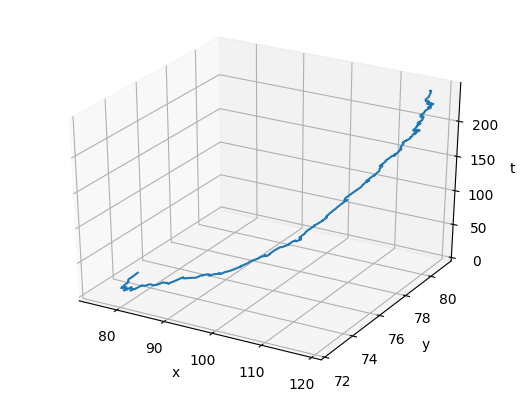
\includegraphics[width=\textwidth]{plots/small/H-GPOMDP-mu.png}
    \end{minipage}
    \vspace{0.5cm}
    \begin{minipage}{0.44\textwidth}
    	\setlength\figureheight{5cm}  
		\setlength\figurewidth{5cm}
		% This file was created by matplotlib2tikz v0.6.16.
\begin{tikzpicture}

\begin{axis}[
xlabel={x},
ylabel={y},
xmin=-50, xmax=200,
ymin=-50, ymax=200,
width=\figurewidth,
height=\figureheight,
tick align=outside,
tick pos=left,
x grid style={white!69.01960784313725!black},
y grid style={white!69.01960784313725!black}
]
\draw[draw=green!50.0!black,fill opacity=0] (axis cs:75.1317003831378,74.6768050837108) ellipse (79.9353395250666 and 79.9382234702847);
\draw[draw=blue,fill opacity=0] (axis cs:110.103388580383,78.5924390364371) ellipse (26.7223871913147 and 35.8134359062225);
\draw[draw=red,fill opacity=0] (axis cs:118.293361504868,80.6952184954765) ellipse (21.7729869463623 and 28.8294594115844);
\addplot [semithick, black, forget plot]
table {%
100 120
120 100
};
\end{axis}

\end{tikzpicture}
    \end{minipage}
    \caption[H-GPOMDP mean value and variance in small environment]{H-GPOMDOP. Left: Mean parameters of the high level policy parameters. Right: The areas in which the $95\%$ of the samples of the high level policy parameters fall into}
    \label{fig:small_h_gpomdp_mu_sigma}
\end{figure}
 
\begin{figure}[t!]
	\centering
    \begin{minipage}{0.55\textwidth}
        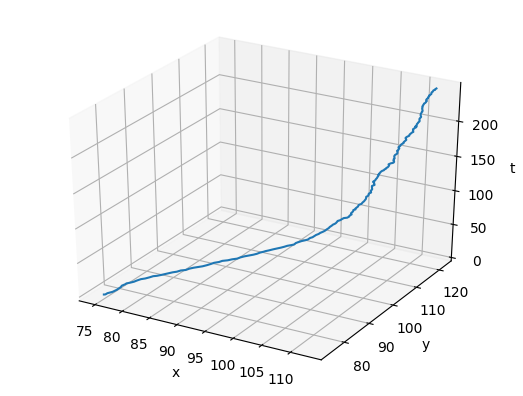
\includegraphics[width=\textwidth]{plots/small/H-PGPE-mu.png}
    \end{minipage}
    \begin{minipage}{0.44\textwidth}
    	\setlength\figureheight{5cm}  
		\setlength\figurewidth{5cm}
		% This file was created by matplotlib2tikz v0.6.16.
\begin{tikzpicture}

\begin{axis}[
xlabel={x},
ylabel={y},
xmin=-50, xmax=200,
ymin=-50, ymax=200,
width=\figurewidth,
height=\figureheight,
tick align=outside,
tick pos=left,
x grid style={white!69.01960784313725!black},
y grid style={white!69.01960784313725!black}
]
\draw[draw=green!50.0!black,fill opacity=0] (axis cs:74.7982194089664,74.5569367094516) ellipse (80.6292347223315 and 78.7779360974279);
\draw[draw=blue,fill opacity=0] (axis cs:105.612897286281,113.672809240917) ellipse (0.229782572592321 and 0.869859091279909);
\draw[draw=red,fill opacity=0] (axis cs:112.53500155361,121.909235094283) ellipse (-0.404669091261131 and -0.00279399170910306);
\addplot [semithick, black, forget plot]
table {%
100 120
120 100
};
\end{axis}

\end{tikzpicture}	
    \end{minipage}
    \caption[H-PGPE mean value and variance in small environment]{H-PGPE. Left: Mean parameters of the high level policy parameters. Right: The areas in which the $95\%$ of the samples of the high level policy parameters fall into}    
    \label{fig:small_h_pgpe_mu_sigma}
\end{figure}


\begin{figure}[t!]
	\centering
    \begin{minipage}{0.55\textwidth}
    	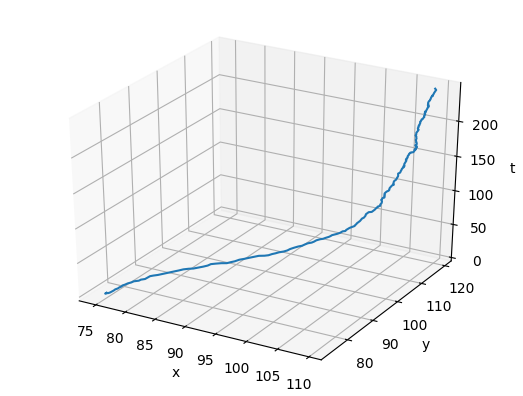
\includegraphics[width=\textwidth]{plots/small/H-PI-mu.png}
    \end{minipage}
    \begin{minipage}{0.44\textwidth}
    	\setlength\figureheight{5cm}  
		\setlength\figurewidth{5cm}
		% This file was created by matplotlib2tikz v0.6.16.
\begin{tikzpicture}

\begin{axis}[
xlabel={x},
ylabel={y},
xmin=-100, xmax=1100,
ymin=-100, ymax=1100,
width=\figurewidth,
height=\figureheight,
tick align=outside,
tick pos=left,
x grid style={white!69.01960784313725!black},
y grid style={white!69.01960784313725!black}
]
\draw[draw=green!50.0!black,fill opacity=0] (axis cs:497.976342114061,498.097206365816) ellipse (506.691499050605 and 507.762144923761);
\draw[draw=blue,fill opacity=0] (axis cs:396.384843374967,397.48448745119) ellipse (3.09446449865456 and 35.1597278943194);
\draw[draw=red,fill opacity=0] (axis cs:401.992682107541,399.80588469616) ellipse (1.14743217377442 and -0.869861990634435);
\addplot [semithick, black, forget plot]
table {%
350 400
450 400
};
\end{axis}

\end{tikzpicture}
    \end{minipage}
    \caption[H-PI mean value and variance in small environment]{H-PI. Left: Mean parameters of the high level policy parameters. Right: The areas in which the $95\%$ of the samples of the high level policy parameters fall into}
    \label{fig:small_h_pi_mu_sigma}
    
\end{figure}

\clearpage

\section{Results in Regular Domain}

The task in the regular ship steering domain possibly is too complex for the flat algorithms due to the larger state-space and random initialization of the ship position. Scaling the discretization from the small to the big environment makes the policy intractable. Therefore, experiments are conducted only with hierarchical algorithms that had a good performance in the small domain: H-PGPE and H-PI. 

The high level controllers use the GPOMDP algorithm to learn a multivariate Gaussian policy with diagonal standard deviation. Policy distribution mean is initialized in the middle of the map, that is $(500, 500)$. The variance of the two dimensions is 255. The algorithm fits every 40 episodes with an adaptive learning rate of 50. Horizon is 100 steps for both the low level and the high level algorithms.

A deterministic policy is constructed by using the absolute values of  weights, that is,  $\pi(x) = \left|\omega\right|x$ for the low level policies. PGPE algorithm learns the distribution over the weights that is initialized with zero mean and $10^{-3}$ variance. The algorithm fits every 10 episodes of the low level controller with an adaptive learning rate of $5\times10{-4}$. The action taken by the low level is a proportional control action for H-PGPE and proportional-integral for H-PI. 

The learning curves of the algorithms are given in Figure~\ref{fig:big_hier_J}. The values are computed with the mean of the objective function for every epoch, averaged for 100 experiments for each algorithm. Curves are slightly less steep than the ones of the smaller domain. This is because the regular domain task is harder. Figure~\ref{fig:big_hier_L} shows the average episode lengths for each epoch, for both algorithms. In the first epochs, low level learns to stay in the map and to follow the referenced angle. Once the high level algorithm detects the gate position, episodes become much shorter, to approximate the shortest path. 

\begin{figure}[t]
	\centering
    \setlength\figureheight{6cm}  
	\setlength\figurewidth{\textwidth}
	% This file was created by matplotlib2tikz v0.6.16.
\begin{tikzpicture}

\definecolor{color0}{rgb}{1,0.498039215686275,0.0549019607843137}

\begin{axis}[
xlabel={epoch},
ylabel={J},
xmin=-1.25, xmax=26.25,
ymin=-99.6868135838367, ymax=-86.1646488743638,
width=\figurewidth,
height=\figureheight,
tick align=outside,
tick pos=left,
ytick distance=2,
x grid style={white!69.01960784313725!black},
y grid style={white!69.01960784313725!black},
legend style={at={(0.03,0.97)}, anchor=north west, draw=white!80.0!black, font=\footnotesize},
legend cell align={left},
legend entries={{H-PGPE},{H-PI}}
]
\addlegendimage{no markers, blue}
\addlegendimage{no markers, color0}
\path [draw=blue, semithick] (axis cs:0,-98.6186432917592)
--(axis cs:0,-99.0721697334062);

\path [draw=blue, semithick] (axis cs:1,-97.3191400856202)
--(axis cs:1,-97.8178021915616);

\path [draw=blue, semithick] (axis cs:2,-97.3278734543125)
--(axis cs:2,-97.8491522869482);

\path [draw=blue, semithick] (axis cs:3,-96.4883726412631)
--(axis cs:3,-97.0522423665752);

\path [draw=blue, semithick] (axis cs:4,-95.3321362008732)
--(axis cs:4,-95.9618640658969);

\path [draw=blue, semithick] (axis cs:5,-93.2854433247004)
--(axis cs:5,-94.043623644619);

\path [draw=blue, semithick] (axis cs:6,-92.0833272273029)
--(axis cs:6,-93.0380850103506);

\path [draw=blue, semithick] (axis cs:7,-91.7688697330869)
--(axis cs:7,-92.640125764855);

\path [draw=blue, semithick] (axis cs:8,-91.4295546914821)
--(axis cs:8,-92.3550538777955);

\path [draw=blue, semithick] (axis cs:9,-90.1366372529003)
--(axis cs:9,-91.1408314789972);

\path [draw=blue, semithick] (axis cs:10,-89.3819097193017)
--(axis cs:10,-90.4569828250573);

\path [draw=blue, semithick] (axis cs:11,-88.6623202015229)
--(axis cs:11,-89.7871428591142);

\path [draw=blue, semithick] (axis cs:12,-88.2028771930043)
--(axis cs:12,-89.2885220246916);

\path [draw=blue, semithick] (axis cs:13,-88.0382573414197)
--(axis cs:13,-88.958562559077);

\path [draw=blue, semithick] (axis cs:14,-87.8354842344783)
--(axis cs:14,-88.7056492880469);

\path [draw=blue, semithick] (axis cs:15,-87.6855425682927)
--(axis cs:15,-88.5232913132147);

\path [draw=blue, semithick] (axis cs:16,-87.4473870237435)
--(axis cs:16,-88.2740763683597);

\path [draw=blue, semithick] (axis cs:17,-87.2568090777906)
--(axis cs:17,-88.0484866995881);

\path [draw=blue, semithick] (axis cs:18,-86.7792927247944)
--(axis cs:18,-87.7952475818047);

\path [draw=blue, semithick] (axis cs:19,-87.5104602783067)
--(axis cs:19,-88.288098992873);

\path [draw=blue, semithick] (axis cs:20,-87.1507000685934)
--(axis cs:20,-87.8272381042379);

\path [draw=blue, semithick] (axis cs:21,-86.8388083556658)
--(axis cs:21,-87.6314974459656);

\path [draw=blue, semithick] (axis cs:22,-87.0965359404103)
--(axis cs:22,-87.9233301161857);

\path [draw=blue, semithick] (axis cs:23,-87.0477044536614)
--(axis cs:23,-87.97837387626);

\path [draw=blue, semithick] (axis cs:24,-87.194786281133)
--(axis cs:24,-87.9462999653316);

\path [draw=blue, semithick] (axis cs:25,-87.2897392480625)
--(axis cs:25,-88.1143129161197);

\path [draw=color0, semithick] (axis cs:0,-98.5796385537277)
--(axis cs:0,-99.0309306475881);

\path [draw=color0, semithick] (axis cs:1,-97.5716316566127)
--(axis cs:1,-97.9918288268185);

\path [draw=color0, semithick] (axis cs:2,-97.0669784243078)
--(axis cs:2,-97.501113678087);

\path [draw=color0, semithick] (axis cs:3,-96.2342627825226)
--(axis cs:3,-96.7869267961619);

\path [draw=color0, semithick] (axis cs:4,-95.0329235446257)
--(axis cs:4,-95.7222100807895);

\path [draw=color0, semithick] (axis cs:5,-93.0937192877062)
--(axis cs:5,-93.8776043635349);

\path [draw=color0, semithick] (axis cs:6,-92.3350837476444)
--(axis cs:6,-93.0417769459607);

\path [draw=color0, semithick] (axis cs:7,-91.4788770484909)
--(axis cs:7,-92.3417237709249);

\path [draw=color0, semithick] (axis cs:8,-91.1310097701006)
--(axis cs:8,-92.047568338441);

\path [draw=color0, semithick] (axis cs:9,-90.4633856769803)
--(axis cs:9,-91.4919649627105);

\path [draw=color0, semithick] (axis cs:10,-89.4641388867949)
--(axis cs:10,-90.4410040316289);

\path [draw=color0, semithick] (axis cs:11,-88.7338270291225)
--(axis cs:11,-89.8049259445917);

\path [draw=color0, semithick] (axis cs:12,-88.072036361087)
--(axis cs:12,-89.075977943898);

\path [draw=color0, semithick] (axis cs:13,-88.0334231036403)
--(axis cs:13,-88.9630553438613);

\path [draw=color0, semithick] (axis cs:14,-87.5037462720889)
--(axis cs:14,-88.4244122807454);

\path [draw=color0, semithick] (axis cs:15,-87.6603391279723)
--(axis cs:15,-88.4998572973396);

\path [draw=color0, semithick] (axis cs:16,-87.3362260245575)
--(axis cs:16,-88.0921312903672);

\path [draw=color0, semithick] (axis cs:17,-87.2567126703445)
--(axis cs:17,-88.0716591757684);

\path [draw=color0, semithick] (axis cs:18,-87.1310731076264)
--(axis cs:18,-88.0129853278574);

\path [draw=color0, semithick] (axis cs:19,-86.960662621279)
--(axis cs:19,-87.7342131976424);

\path [draw=color0, semithick] (axis cs:20,-87.4994605608238)
--(axis cs:20,-88.2187986048138);

\path [draw=color0, semithick] (axis cs:21,-86.9885281246732)
--(axis cs:21,-87.8190471228839);

\path [draw=color0, semithick] (axis cs:22,-87.1373384630533)
--(axis cs:22,-87.8540316644523);

\path [draw=color0, semithick] (axis cs:23,-87.320752285901)
--(axis cs:23,-88.0645632405074);

\path [draw=color0, semithick] (axis cs:24,-86.9449738682615)
--(axis cs:24,-87.8696912413971);

\path [draw=color0, semithick] (axis cs:25,-87.3435372012375)
--(axis cs:25,-88.1321930489828);

\addplot [semithick, blue, forget plot]
table {%
0 -98.8454065125827
1 -97.5684711385909
2 -97.5885128706303
3 -96.7703075039191
4 -95.6470001333851
5 -93.6645334846597
6 -92.5607061188267
7 -92.2044977489709
8 -91.8923042846388
9 -90.6387343659487
10 -89.9194462721795
11 -89.2247315303186
12 -88.745699608848
13 -88.4984099502484
14 -88.2705667612626
15 -88.1044169407537
16 -87.8607316960516
17 -87.6526478886894
18 -87.2872701532995
19 -87.8992796355898
20 -87.4889690864157
21 -87.2351529008157
22 -87.509933028298
23 -87.5130391649607
24 -87.5705431232323
25 -87.7020260820911
};
\addplot [semithick, color0, forget plot]
table {%
0 -98.8052846006579
1 -97.7817302417156
2 -97.2840460511974
3 -96.5105947893422
4 -95.3775668127076
5 -93.4856618256205
6 -92.6884303468026
7 -91.9103004097079
8 -91.5892890542708
9 -90.9776753198454
10 -89.9525714592119
11 -89.2693764868571
12 -88.5740071524925
13 -88.4982392237508
14 -87.9640792764171
15 -88.0800982126559
16 -87.7141786574624
17 -87.6641859230565
18 -87.5720292177419
19 -87.3474379094607
20 -87.8591295828188
21 -87.4037876237786
22 -87.4956850637528
23 -87.6926577632042
24 -87.4073325548293
25 -87.7378651251101
};
\end{axis}

\end{tikzpicture}
    \caption[J comparison, regular environment]{Average of objective function of the hierarchical algorithms at every epoch}
    \label{fig:big_hier_J}
\end{figure}
\begin{figure}[t]
    \setlength\figureheight{6cm}  
	\setlength\figurewidth{\textwidth}
	% This file was created by matplotlib2tikz v0.6.16.
\begin{tikzpicture}

\definecolor{color0}{rgb}{1,0.498039215686275,0.0549019607843137}
\definecolor{color1}{rgb}{0.580392156862745,0.403921568627451,0.741176470588235}

\begin{axis}[
xlabel={epoch},
ylabel={episode length},
xmin=-1.25, xmax=26.25,
ymin=-34.915452394257, ymax=1141.7474948898,
width=\figurewidth,
height=\figureheight,
tick align=outside,
tick pos=left,
x grid style={white!69.01960784313725!black},
y grid style={white!69.01960784313725!black}
]
\path [draw=blue, semithick] (axis cs:0,81.0911760668363)
--(axis cs:0,79.7708239331638);

\path [draw=blue, semithick] (axis cs:1,489.404089545043)
--(axis cs:1,426.197910454957);

\path [draw=blue, semithick] (axis cs:2,1088.2628154678)
--(axis cs:2,883.186184532202);

\path [draw=blue, semithick] (axis cs:3,902.729243554014)
--(axis cs:3,668.031756445986);

\path [draw=blue, semithick] (axis cs:4,538.649445355297)
--(axis cs:4,388.479554644704);

\path [draw=blue, semithick] (axis cs:5,360.585648488226)
--(axis cs:5,256.607351511774);

\path [draw=blue, semithick] (axis cs:6,206.965204754822)
--(axis cs:6,168.017795245178);

\path [draw=blue, semithick] (axis cs:7,169.231441872846)
--(axis cs:7,133.929558127155);

\path [draw=blue, semithick] (axis cs:8,133.475028224666)
--(axis cs:8,114.202971775334);

\path [draw=blue, semithick] (axis cs:9,120.197500073287)
--(axis cs:9,102.460499926713);

\path [draw=blue, semithick] (axis cs:10,104.727491148319)
--(axis cs:10,94.9935088516812);

\path [draw=blue, semithick] (axis cs:11,108.924620800781)
--(axis cs:11,95.2993791992188);

\path [draw=blue, semithick] (axis cs:12,104.255991538558)
--(axis cs:12,93.2330084614424);

\path [draw=blue, semithick] (axis cs:13,98.0292641895068)
--(axis cs:13,92.0547358104933);

\path [draw=blue, semithick] (axis cs:14,98.8711748590563)
--(axis cs:14,90.1158251409437);

\path [draw=blue, semithick] (axis cs:15,93.3654467977495)
--(axis cs:15,89.5665532022504);

\path [draw=blue, semithick] (axis cs:16,97.5575558096076)
--(axis cs:16,90.2624441903923);

\path [draw=blue, semithick] (axis cs:17,97.9323236248251)
--(axis cs:17,91.0486763751749);

\path [draw=blue, semithick] (axis cs:18,95.5247837818183)
--(axis cs:18,90.2502162181817);

\path [draw=blue, semithick] (axis cs:19,94.023289405138)
--(axis cs:19,89.856710594862);

\path [draw=blue, semithick] (axis cs:20,92.2067689802821)
--(axis cs:20,89.3982310197179);

\path [draw=blue, semithick] (axis cs:21,93.391101891151)
--(axis cs:21,89.895898108849);

\path [draw=blue, semithick] (axis cs:22,93.3524553428036)
--(axis cs:22,90.0975446571963);

\path [draw=blue, semithick] (axis cs:23,97.7341276584202)
--(axis cs:23,88.6568723415798);

\path [draw=blue, semithick] (axis cs:24,90.3209027734668)
--(axis cs:24,88.8900972265332);

\path [draw=blue, semithick] (axis cs:25,92.5221037823311)
--(axis cs:25,89.4808962176688);

\path [draw=color0, semithick] (axis cs:0,80.8898148348609)
--(axis cs:0,79.4681851651391);

\path [draw=color0, semithick] (axis cs:1,439.120094554962)
--(axis cs:1,377.640905445038);

\path [draw=color0, semithick] (axis cs:2,1032.95442974765)
--(axis cs:2,842.891570252345);

\path [draw=color0, semithick] (axis cs:3,856.783597826666)
--(axis cs:3,675.807402173334);

\path [draw=color0, semithick] (axis cs:4,591.144024461649)
--(axis cs:4,447.192975538351);

\path [draw=color0, semithick] (axis cs:5,320.693359972832)
--(axis cs:5,257.479640027168);

\path [draw=color0, semithick] (axis cs:6,210.400236336701)
--(axis cs:6,167.771763663299);

\path [draw=color0, semithick] (axis cs:7,151.610366773235)
--(axis cs:7,124.861633226765);

\path [draw=color0, semithick] (axis cs:8,127.940874876469)
--(axis cs:8,112.022125123531);

\path [draw=color0, semithick] (axis cs:9,118.527082951398)
--(axis cs:9,104.114917048602);

\path [draw=color0, semithick] (axis cs:10,105.946442170183)
--(axis cs:10,97.0455578298172);

\path [draw=color0, semithick] (axis cs:11,105.632499394661)
--(axis cs:11,93.9745006053392);

\path [draw=color0, semithick] (axis cs:12,98.3736022287574)
--(axis cs:12,92.9923977712426);

\path [draw=color0, semithick] (axis cs:13,95.7685447996079)
--(axis cs:13,91.4294552003921);

\path [draw=color0, semithick] (axis cs:14,96.2767949771307)
--(axis cs:14,89.8092050228693);

\path [draw=color0, semithick] (axis cs:15,92.2745034094563)
--(axis cs:15,89.8884965905437);

\path [draw=color0, semithick] (axis cs:16,93.3287433870181)
--(axis cs:16,90.1812566129819);

\path [draw=color0, semithick] (axis cs:17,91.8728528575949)
--(axis cs:17,89.3481471424052);

\path [draw=color0, semithick] (axis cs:18,93.264917045919)
--(axis cs:18,89.6680829540809);

\path [draw=color0, semithick] (axis cs:19,92.7231665552644)
--(axis cs:19,89.4238334447355);

\path [draw=color0, semithick] (axis cs:20,95.5063672858701)
--(axis cs:20,90.08563271413);

\path [draw=color0, semithick] (axis cs:21,91.2686813137062)
--(axis cs:21,89.0083186862937);

\path [draw=color0, semithick] (axis cs:22,90.8035134720861)
--(axis cs:22,88.650486527914);

\path [draw=color0, semithick] (axis cs:23,92.3091956446672)
--(axis cs:23,89.1378043553328);

\path [draw=color0, semithick] (axis cs:24,93.5936523439909)
--(axis cs:24,89.6223476560091);

\path [draw=color0, semithick] (axis cs:25,92.3530804421264)
--(axis cs:25,89.4229195578736);

\path [draw=color1, semithick] (axis cs:0,21.4947729722544)
--(axis cs:0,18.5692270277456);

\path [draw=color1, semithick] (axis cs:1,177.082150179711)
--(axis cs:1,110.338849820289);

\path [draw=color1, semithick] (axis cs:2,340.643305773912)
--(axis cs:2,183.941694226088);

\path [draw=color1, semithick] (axis cs:3,360.332570573641)
--(axis cs:3,215.438429426359);

\path [draw=color1, semithick] (axis cs:4,277.493936776158)
--(axis cs:4,168.064063223841);

\path [draw=color1, semithick] (axis cs:5,257.145558889606)
--(axis cs:5,152.756441110393);

\path [draw=color1, semithick] (axis cs:6,228.023642986969)
--(axis cs:6,109.413357013031);

\path [draw=color1, semithick] (axis cs:7,279.080792455482)
--(axis cs:7,74.3622075445179);

\path [draw=color1, semithick] (axis cs:8,251.4236248622)
--(axis cs:8,66.5243751377995);

\path [draw=color1, semithick] (axis cs:9,231.433418374939)
--(axis cs:9,39.5205816250608);

\path [draw=color1, semithick] (axis cs:10,200.793117170882)
--(axis cs:10,59.4268828291176);

\path [draw=color1, semithick] (axis cs:11,173.736892736264)
--(axis cs:11,75.6181072637357);

\path [draw=color1, semithick] (axis cs:12,120.422034306393)
--(axis cs:12,64.6239656936068);

\path [draw=color1, semithick] (axis cs:13,154.479879676207)
--(axis cs:13,61.065120323793);

\path [draw=color1, semithick] (axis cs:14,207.460464821122)
--(axis cs:14,33.8015351788782);

\path [draw=color1, semithick] (axis cs:15,206.070374646037)
--(axis cs:15,35.3876253539627);

\path [draw=color1, semithick] (axis cs:16,215.924292317934)
--(axis cs:16,28.9867076820658);

\path [draw=color1, semithick] (axis cs:17,98.0872237981273)
--(axis cs:17,52.4477762018727);

\path [draw=color1, semithick] (axis cs:18,87.9319820355879)
--(axis cs:18,58.4950179644121);

\path [draw=color1, semithick] (axis cs:19,79.9470258352977)
--(axis cs:19,57.9949741647023);

\path [draw=color1, semithick] (axis cs:20,177.12603638901)
--(axis cs:20,26.7319636109902);

\path [draw=color1, semithick] (axis cs:21,127.835610127343)
--(axis cs:21,41.2623898726565);

\path [draw=color1, semithick] (axis cs:22,93.3663605082555)
--(axis cs:22,57.6176394917445);

\path [draw=color1, semithick] (axis cs:23,80.6185662904916)
--(axis cs:23,59.8684337095084);

\path [draw=color1, semithick] (axis cs:24,79.6719092223636)
--(axis cs:24,60.0990907776364);

\path [draw=color1, semithick] (axis cs:25,81.8456657834132)
--(axis cs:25,61.6783342165868);

\addplot [semithick, blue, forget plot]
table {%
0 80.4310000000001
1 457.801
2 985.7245
3 785.3805
4 463.5645
5 308.5965
6 187.4915
7 151.5805
8 123.839
9 111.329
10 99.8605
11 102.112
12 98.7445
13 95.042
14 94.4935
15 91.466
16 93.91
17 94.4905
18 92.8875
19 91.94
20 90.8025
21 91.6435
22 91.725
23 93.1955
24 89.6055
25 91.0015
};
\addplot [semithick, color0, forget plot]
table {%
0 80.179
1 408.3805
2 937.923
3 766.2955
4 519.1685
5 289.0865
6 189.086
7 138.236
8 119.9815
9 111.321
10 101.496
11 99.8035
12 95.683
13 93.599
14 93.043
15 91.0815
16 91.755
17 90.6105
18 91.4665
19 91.0735
20 92.796
21 90.1385
22 89.727
23 90.7235
24 91.608
25 90.888
};
\addplot [semithick, color1, forget plot]
table {%
0 20.032
1 143.7105
2 262.2925
3 287.8855
4 222.779
5 204.951
6 168.7185
7 176.7215
8 158.974
9 135.477
10 130.11
11 124.6775
12 92.523
13 107.7725
14 120.631
15 120.729
16 122.4555
17 75.2675
18 73.2135
19 68.971
20 101.929
21 84.549
22 75.492
23 70.2435
24 69.8855
25 71.762
};
\end{axis}

\end{tikzpicture}
    \caption[Episode length comparison, regular environment]{Average episode lengths of hierarchical algorithms at every epoch}
    \label{fig:big_hier_L}
\end{figure}

\clearpage

Figure~\ref{fig:big_traj_h_pgpe} depicts the trajectories of the last 5 episodes of the epochs 0, 3, 12 and 24 for the H-PGPE algorithm and Figure~\ref{fig:big_traj_h_pi} shows that of the H-PI algorithm. The trajectories start at random points as the high level task requires. In both figures we observe a stroll around the gate at the last steps. This is because the ship starts at random points and the gate is in the middle of the map. These characteristics of the regular domain eliminate the possibility of placing the reference position behind the gate. Moreover, when the ship is almost reaching the gate, low level policy performance is lousy. We observe a negative peak in the low level intrinsic reward as the angle difference jumps from 0 to $\pi$ while the ship trespass the reference point.


\figuretraj{big}{H-PGPE}{H-PGPE trajectories, regular environment}{hierarchical algorithm with PGPE in the low level, last 5 trajectories of the epochs}{fig:big_traj_h_pgpe}
\figuretraj{big}{H-PI}{H-PI trajectories, regular environment}{hierarchical algorithm with PGPE in the low level, with integral action, last 5 trajectories of the epochs}{fig:big_traj_h_pi}

 
 The average of the parameters of the hierarchical algorithm with PGPE in the low level (H-PGPE) is shown in Figure~\ref{fig:big_h_pgpe_mu_sigma}. Figure~\ref{fig:big_h_pi_mu_sigma} demonstrates the same observations for hierarchical algorithm with PGPE learning a policy with integral action in the low level (H-PI). We observe that both algorithms are able to identify the gate position quite fast, almost as fast as they identified the gate in the small domain. The fast convergence is explained by the fact that the position of the gate is near to the middle of the map and the initial distribution of the high level is centered in there. 

\begin{figure}[t]
	\centering
    \begin{minipage}{0.55\textwidth}
        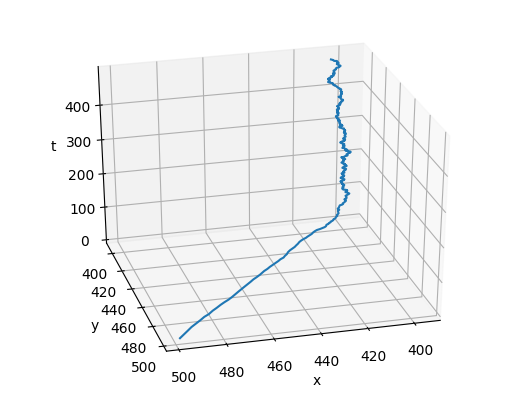
\includegraphics[width=\textwidth]{plots/big/H-PGPE-mu.png}
    \end{minipage}
    \begin{minipage}{0.44\textwidth}
    	\setlength\figureheight{5cm}  
		\setlength\figurewidth{5cm}
		% This file was created by matplotlib2tikz v0.6.16.
\begin{tikzpicture}

\begin{axis}[
xlabel={x},
ylabel={y},
xmin=-50, xmax=200,
ymin=-50, ymax=200,
width=\figurewidth,
height=\figureheight,
tick align=outside,
tick pos=left,
x grid style={white!69.01960784313725!black},
y grid style={white!69.01960784313725!black}
]
\draw[draw=green!50.0!black,fill opacity=0] (axis cs:74.7982194089664,74.5569367094516) ellipse (80.6292347223315 and 78.7779360974279);
\draw[draw=blue,fill opacity=0] (axis cs:105.612897286281,113.672809240917) ellipse (0.229782572592321 and 0.869859091279909);
\draw[draw=red,fill opacity=0] (axis cs:112.53500155361,121.909235094283) ellipse (-0.404669091261131 and -0.00279399170910306);
\addplot [semithick, black, forget plot]
table {%
100 120
120 100
};
\end{axis}

\end{tikzpicture}
    \end{minipage}
    \caption[H-PGPE mean value and variance in regular environment]{H-PGPE in regular domain. Left: Mean parameters of the high level policy parameters. Right: The areas in which the $95\%$ of the samples of the high level policy parameters fall into}
    \label{fig:big_h_pgpe_mu_sigma}
\end{figure}


\begin{figure}[t]
	\centering
    \begin{minipage}{0.55\textwidth}
    	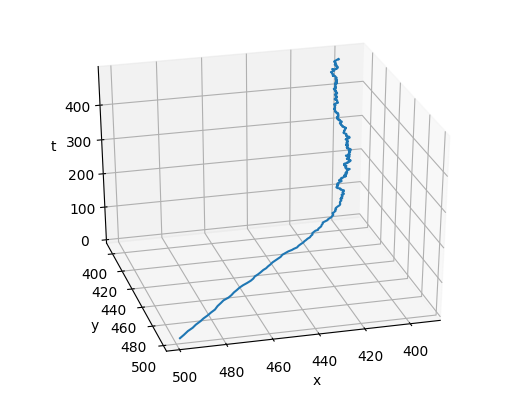
\includegraphics[width=\textwidth]{plots/big/H-PI-mu.png}
    \end{minipage}
    \begin{minipage}{0.44\textwidth}
    	\setlength\figureheight{5cm}  
		\setlength\figurewidth{5cm}
		% This file was created by matplotlib2tikz v0.6.16.
\begin{tikzpicture}

\begin{axis}[
xlabel={x},
ylabel={y},
xmin=-100, xmax=1100,
ymin=-100, ymax=1100,
width=\figurewidth,
height=\figureheight,
tick align=outside,
tick pos=left,
x grid style={white!69.01960784313725!black},
y grid style={white!69.01960784313725!black}
]
\draw[draw=green!50.0!black,fill opacity=0] (axis cs:497.976342114061,498.097206365816) ellipse (506.691499050605 and 507.762144923761);
\draw[draw=blue,fill opacity=0] (axis cs:396.384843374967,397.48448745119) ellipse (3.09446449865456 and 35.1597278943194);
\draw[draw=red,fill opacity=0] (axis cs:401.992682107541,399.80588469616) ellipse (1.14743217377442 and -0.869861990634435);
\addplot [semithick, black, forget plot]
table {%
350 400
450 400
};
\end{axis}

\end{tikzpicture}
    \end{minipage}
    \caption[H-PI mean value and variance in regular environment]{H-PI in regular domain. Left: Mean parameters of the high level policy parameters. Right: The areas in which the $95\%$ of the samples of the high level policy parameters fall into}
    \label{fig:big_h_pi_mu_sigma}
\end{figure}


